\documentclass[a4paper,12pt]{article}
\usepackage[margin=22mm]{geometry}
\usepackage[utf8]{vietnam}
\usepackage{graphicx}
\usepackage{amsmath}
\usepackage{bm}
\usepackage{amsxtra,amssymb,latexsym,amscd,amsthm}
\usepackage{fancyhdr}
\usepackage{float}
\usepackage[plain]{algorithm}
\usepackage{mathtools}
\usepackage{blindtext}
\usepackage{titlesec}
\usepackage{filecontents}
\usepackage{listings}
\usepackage{enumitem}
\usepackage{xcolor, soul}
\usepackage{setspace}
\usepackage{indentfirst}
\usepackage[hidelinks]{hyperref}
\usepackage{blindtext}
\usepackage{tikz}
\usepackage{indentfirst}
\usepackage{ragged2e}
%\addtokomafont{disposition}{\boldmath}% use bold math in titles
\usepackage{natbib}
\usepackage{filecontents,hyperref}
\usepackage{enumitem}
\usepackage{subfig}
\usepackage{tabularray}
\usepackage{array}
\usepackage{booktabs}

\definecolor{codegreen}{rgb}{0,0.6,0}
\definecolor{codegray}{rgb}{0.5,0.5,0.5}
\definecolor{codepurple}{rgb}{0.58,0,0.82}
\definecolor{backcolour}{rgb}{0.95,0.95,0.92}

\lstdefinestyle{mystyle}{
    backgroundcolor=\color{backcolour},   
    commentstyle=\color{codegreen},
    keywordstyle=\color{magenta},
    numberstyle=\tiny\color{codegray},
    stringstyle=\color{codepurple},
    basicstyle=\ttfamily\footnotesize,
    breakatwhitespace=false,         
    breaklines=true,                 
    captionpos=b,                    
    keepspaces=true,                 
    numbers=left,                    
    numbersep=5pt,                  
    showspaces=false,                
    showstringspaces=false,
    showtabs=false,                  
    tabsize=2
}

\lstset{style=mystyle}

%\setlength{\parindent}{0pt}

\begin{document}
\setcounter{secnumdepth}{5}
\setstretch{1.2}
\begin{titlepage}
\begin{center}
    \textbf{\large TRƯỜNG ĐẠI HỌC CÔNG NGHỆ THÔNG TIN} \\
    {\large KHOA KHOA HỌC MÁY TÍNH\vfill
    NHẬP MÔN THỊ GIÁC MÁY TÍNH - CS231\vfill
    
\includegraphics[width=0.3\textwidth]{graphics/UIT.png} \vfill
    \textbf{\Large BÁO CÁO ĐỒ ÁN}\\
    \smallskip
    \textbf{\Large ĐỀ TÀI: NHẬN DIỆN NGƯỜI ĐI BỘ}\vfill
    GV hướng dẫn: TS. Mai Tiến Dũng \vfill
    Nhóm thực hiện: \vspace{0.5cm} \\
    \begin{tabular}{l r}
        1. Nguyễn Như Hà & 21522028 \\
        2. Nguyễn Thị Thanh Lan & 21521065 \\
        3. Bùi Lê Khánh Linh & 21522284 \\
    \end{tabular} \vfill
    TPHCM, ngày 2 tháng 7 năm 2023
    }
\end{center}
\end{titlepage}
\begin{titlepage}
    \begin{center}
        \textbf{\Large Lời cảm ơn}
    \end{center}
    Nhóm chúng em xin gửi lời cảm ơn chân thành đến T.S Mai Tiến Dũng - Giảng viên khoa Khoa học máy tính, trường Đại học Công nghệ thông tin, Đại học Quốc gia Thành phố Hồ Chí Minh, phụ trách lớp CS231.N21.KHCL - Môn Nhập môn thị giác máy tính, trong thời gian qua đã tận tình truyền đạt và giảng dạy những kiến thức, kỹ năng vô cùng hữu ích về thị giác máy tính.
    \vspace{5mm}
    \\
    Trong quá trình thực hiện đồ án môn học, mặc dù nhóm đã cố gắng nhưng chắc chắn sẽ không tránh được những sai sót không đáng có. Qua buổi trình bày trên lớp thì nhóm đã nhận được những góp ý của thầy và câu hỏi của các bạn đồng thời chúng em đã thực hiện những sửa đổi để bài báo cáo trở nên hoàn thiện. Nhờ những đóng góp đó mà nhóm chúng em tích lũy thêm nhiều kinh nghiệm và kiến thức. Qua môn học này, chúng em đã được củng cố không chỉ kiến thức môn học mà phát triển kỹ năng thuyết trình, kỹ năng tìm kiếm tài liệu. Chúng em xin chân thành cảm ơn!
    \begin{flushright}
        Thành phố Hồ Chí Minh, tháng 7 năm 2023
    \end{flushright}
\end{titlepage}
\tableofcontents
\pagebreak

\section{Tổng quan}
\subsection{Giới thiệu về bài toán Object Detection}
Trong phần này nhóm sẽ giới thiệu về thị giác máy tính (Computer Vision – CV) và bài toán Object Detection \cite{objectdetection}.

Thị giác máy tính có thể giải thích đơn giản như sau: Đó là một lĩnh vực của trí tuệ nhân tạo (AI) và khoa học máy tính liên quan đến việc xử lý, phân tích và hiểu các hình ảnh và video. Nó tập trung vào việc tạo ra các thuật toán và phương pháp để cho máy tính có khả năng nhìn và hiểu thế giới xung quanh giống như con người bình thường.

Một số bài toán trong lĩnh vực này bao gồm Image classification, Classification with Localization, Object Detection, Instance Segmentation.

\graphicspath{{figures/}}
\begin{figure}[h!]
  \centering
  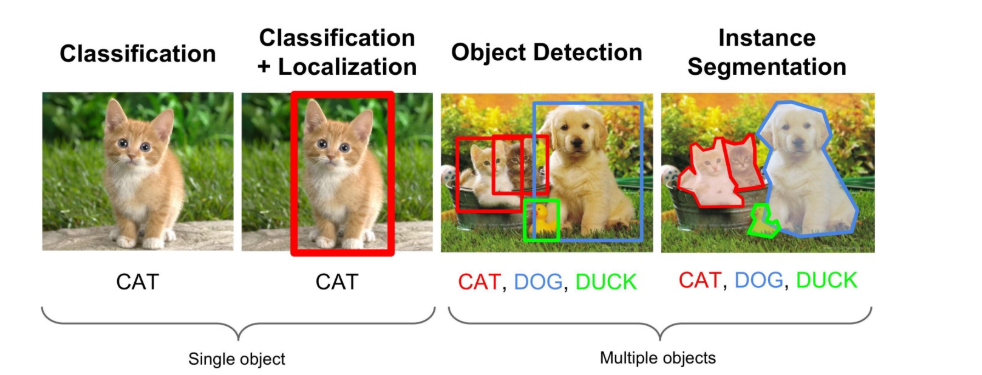
\includegraphics[scale=0.4]{graphics/Hinh1.png}
  \caption{Một số bài toán trong lĩnh vực CV}
\end{figure}

% \begin{center}
%     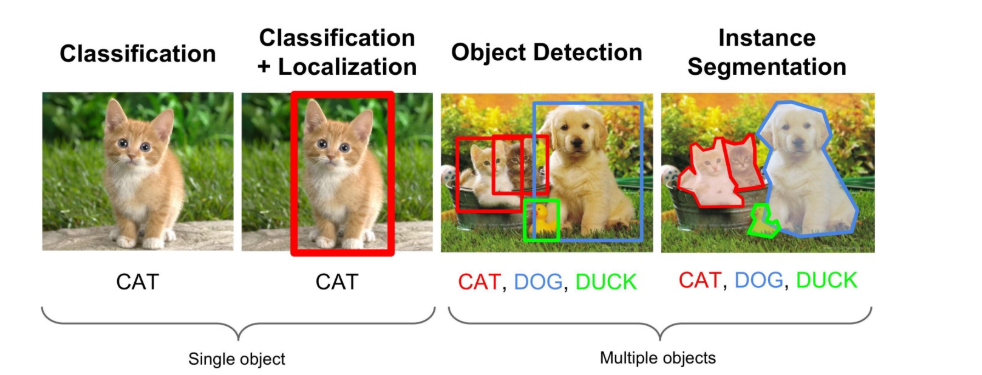
\includegraphics[scale=0.45]{graphics/Hinh1.png}
% \end{center}

\graphicspath{{figures/}}
\begin{figure}[h!]
  \centering
  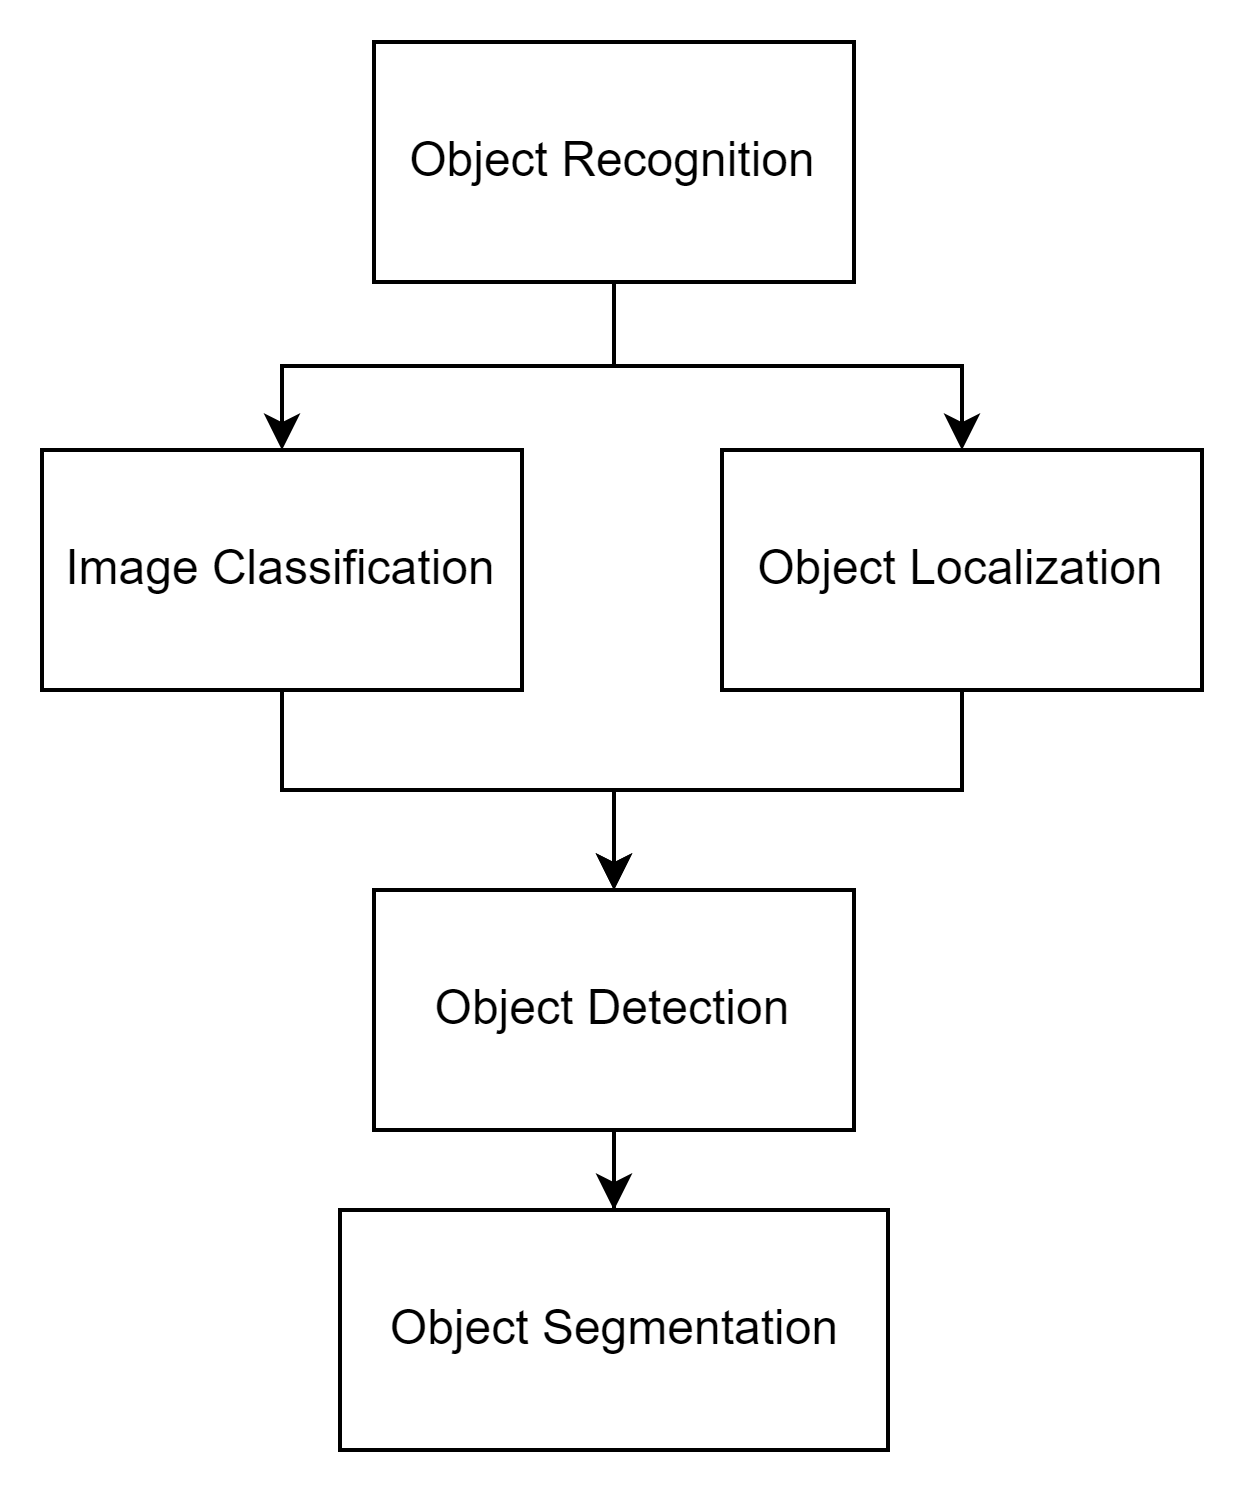
\includegraphics[scale=0.18]{graphics/general.png}
  \caption{Sơ lược mối liên hệ giữa các tác vụ trong thị giác máy tính}
\end{figure}
Trong lĩnh vực Thị giác máy tính và Trí tuệ nhân tạo, bài toán Object Detection đã trở thành một chủ đề quan trọng và hấp dẫn. Bài toán này đóng vai trò cốt lõi trong việc xác định và định vị các đối tượng trong một hình ảnh hoặc video. Hiểu và giải quyết bài toán này mang lại nhiều ứng dụng thực tế, như trong lĩnh vực tự lái xe, giám sát an ninh, phân loại hình ảnh và nhận dạng khuôn mặt.

Bài toán Object Detection (nhận diện vật thể) trong đó mục tiêu là xác định và phân loại các vật thể xuất hiện trong hình ảnh hoặc video. Bài toán này đòi hỏi mô hình máy tính phải có khả năng phát hiện và định vị vật thể trong hình ảnh, đồng thời gán nhãn cho chúng thuộc các lớp vật thể khác nhau. Ta phải đối mặt với các thách thức như sự biến đổi về kích thước, hình dạng và góc nhìn của vật thể, đồng thời còn phải xử lý các vấn đề như nhiễu, che khuất và độ phức tạp của môi trường.

\graphicspath{{figures/}}
\begin{figure}[h!]
  \centering
  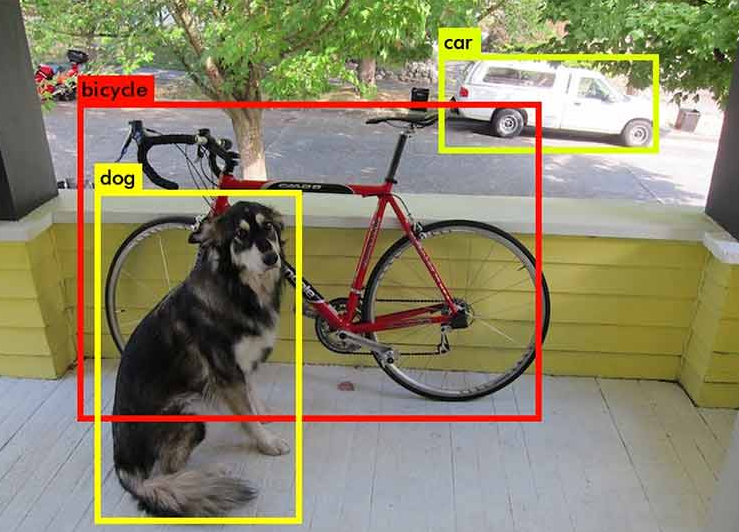
\includegraphics[scale=0.4]{graphics/object detection.png}
  \caption{Ví dụ về bài toán Object Detection}
\end{figure}

Một số phương pháp truyền thống đã được sử dụng cho bài toán Object Detection bao gồm phân đoạn ảnh, phát hiện biên, phương pháp dựa trên cửa sổ trượt và phương pháp dựa trên các đặc trưng cục bộ. Mặc dù các phương pháp này có những ưu điểm riêng, nhưng chúng cũng gặp phải một số hạn chế, đặc biệt là khi xử lý các hình ảnh có nhiều đối tượng và độ phức tạp cao.

Với sự phát triển của Deep Learning, các mô hình dựa trên mạng neural đã mang lại những bước tiến đáng kể trong việc giải quyết bài toán Object Detection, kể đến như R-CNN, Fast R-CNN, Faster R-CNN và YOLO. Những mô hình này sử dụng các kiến trúc mạng neural phức tạp để xác định và định vị các đối tượng một cách hiệu quả trong hình ảnh.

Ứng dụng của Object Detection rất đa dạng và phong phú. Trong lĩnh vực tự lái xe, Object Detection được sử dụng để phát hiện và phản ứng với các đối tượng như xe, người đi bộ, biển báo giao thông và điều kiện đường. Trong giám sát an ninh, nó có thể giúp xác định và theo dõi các đối tượng đáng ngờ trong các hình ảnh hoặc video giám sát. Bên cạnh đó, Object Detection cũng có thể áp dụng trong các lĩnh vực như phân loại hình ảnh và nhận dạng khuôn mặt.

\graphicspath{{figures/}}
\begin{figure}[h!]
  \centering
  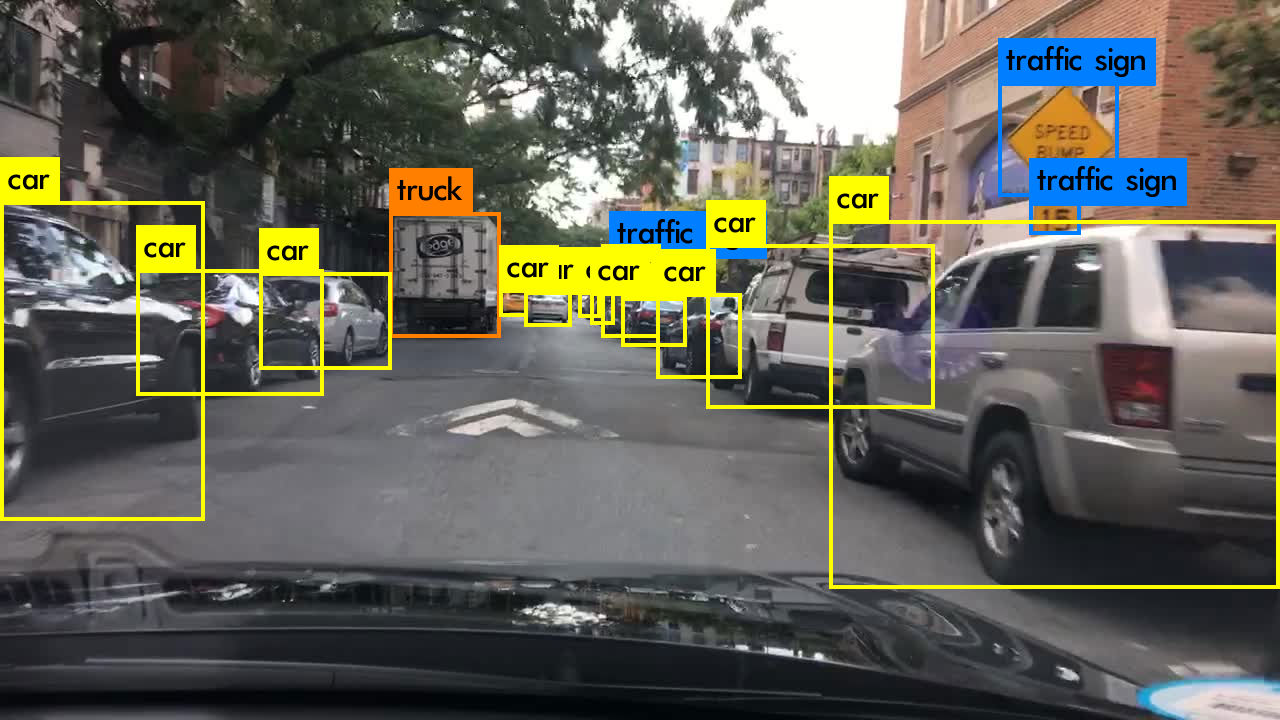
\includegraphics[scale=0.3]{graphics/Object Detection in Autonomous Driving.jpg}
  \caption{Object Detection ứng dụng trong xe tự hành}
\end{figure}

Với những tiến bộ trong Deep Learning và sự phát triển của công nghệ, bài toán Object Detection đang trở thành một lĩnh vực nghiên cứu hứa hẹn. Việc nghiên cứu và áp dụng những phương pháp hiện đại trong bài toán này có thể mang lại những ứng dụng thực tiễn mạnh mẽ trong tương lai.

\subsection{Giới thiệu về đồ án}
Đồ án này tập trung vào bài toán Pedestrian Detection, một đề tài không còn quá xa lạ đối với những người đã và đang tiếp cận bài toán Object Detection. Bài toán này nhằm xác định và định vị vị trí của người đi bộ trong các hình ảnh hoặc video, có ứng dụng rộng rãi trong nhiều lĩnh vực như giám sát an ninh, xe tự hành và các hệ thống nhận diện. Đồ án sẽ trình bày hai cách tiếp cận khác nhau để giải quyết bài toán Pedestrian Detection, đó là sử dụng mô hình HOG+SVM và mô hình Faster R-CNN.

\graphicspath{{figures/}}
\begin{figure}[h!]
  \centering
  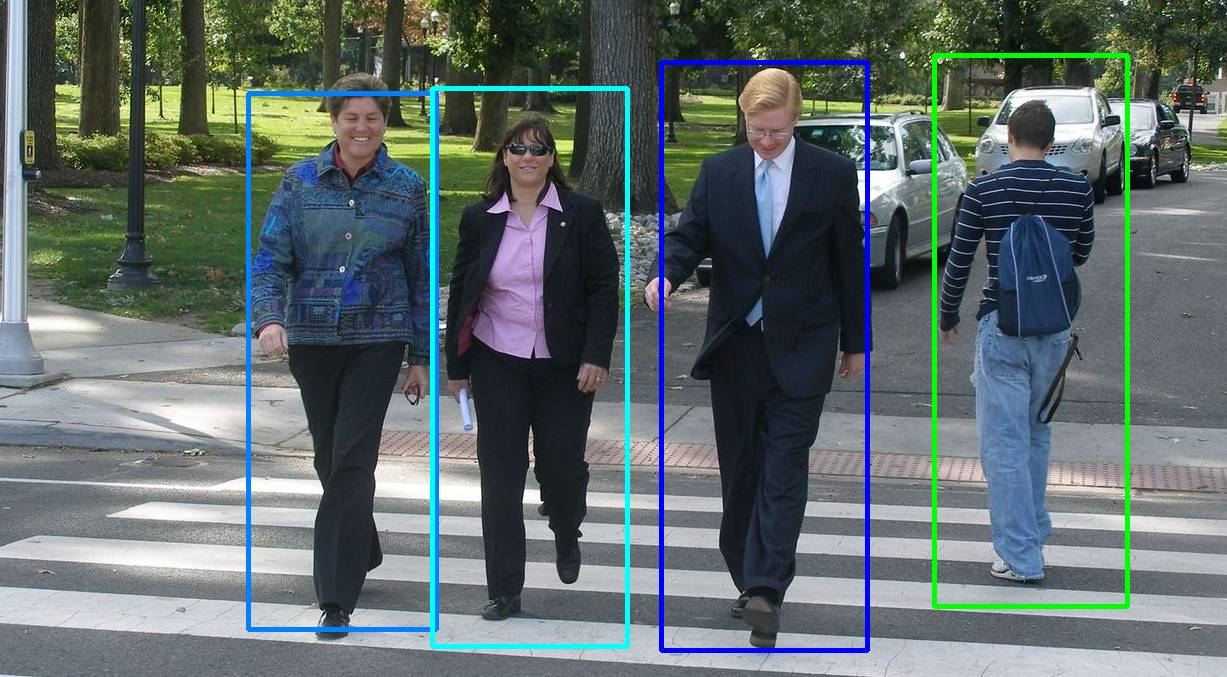
\includegraphics[scale=0.39]{graphics/Hinh2.jpg}
  \caption{Nhận diện người đi bộ (Pedestrian Detection)}
\end{figure}

Cách tiếp cận đầu tiên của nhóm sẽ sử dụng mô hình HOG (Histogram of Oriented Gradients) kết hợp với SVM (Support Vector Machine). Mô hình HOG là một phương pháp biểu diễn đặc trưng được sử dụng để mô tả hình dạng của đối tượng. Bằng cách tính toán gradient của các khối hình ảnh, HOG tạo ra một biểu diễn đặc trưng mô tả sự phân bố các đường cạnh và hướng của hình ảnh. Sau đó, SVM được sử dụng để phân loại đối tượng có chứa người đi bộ hoặc không. Mô hình HOG+SVM đã được chứng minh là hiệu quả trong việc phát hiện người đi bộ trong ảnh tĩnh.

Cách tiếp cận thứ hai sẽ sử dụng mô hình Faster R-CNN (Region-based Convolutional Neural Network). Mô hình này kết hợp giữa hai thành phần chính là mạng neural tích chập (CNN) và mạng neural nhận diện vùng đặc trưng (R-CNN). Với Faster R-CNN, đầu tiên, một mạng CNN được sử dụng để trích xuất các đặc trưng từ hình ảnh. Sau đó, mạng R-CNN được sử dụng để phát hiện và định vị vùng chứa người đi bộ dựa trên các đặc trưng đã trích xuất. Mô hình Faster R-CNN có khả năng tự động học các đặc trưng phù hợp với bài toán Pedestrian Detection, đồng thời cung cấp độ chính xác cao.

Trong quá trình thực hiện đồ án, nhóm sẽ tiến hành huấn luyện và đánh giá hiệu suất của cả hai cách tiếp cận trên tập dữ liệu đã được gán nhãn, chứa các hình ảnh có chứa và không chứa người đi bộ. Hiệu suất của các mô hình sẽ được đánh giá dựa trên độ đo mAP.

\subsection{Lý do chọn đề tài}
Đề tài này được nhóm chọn dựa trên sự quan tâm từ việc ứng dụng nhận dạng đối tượng có thể mang lại trong các lĩnh vực như an ninh, xử lý ảnh, và tự động hóa công nghiệp. Mục tiêu của đồ án nhận diện người đi bộ này là phân loại và xác định vị trí chính xác của các người đi bộ trong hình ảnh để tạo nền tảng cho việc xây dựng các ứng dụng thông minh dựa trên thị giác máy tính.

Một ứng dụng cho bài toán nhận diện người đi bộ vô cùng thực tế mà nhóm đã được thầy góp ý là việc ứng dụng nó trong các siêu thị, trung tâm thương mại để quan sát vị trí nào mà khách hàng tập trung nhiều nhất để từ đó đưa ra các biện pháp tối ưu hóa trải nghiệm mua sắm và cải thiện quản lý cửa hàng. Bằng cách sử dụng hệ thống nhận diện người đi bộ, siêu thị và trung tâm thương mại có thể phân tích và đếm số lượng khách hàng tại các khu vực khác nhau trong cửa hàng. Thông qua việc phân tích dữ liệu, họ có thể xác định vị trí nào thu hút nhiều khách hàng nhất và tạo ra các chiến lược trưng bày sản phẩm hiệu quả để tăng doanh số bán hàng.
\pagebreak
\begin{figure}[h!]
  \centering
  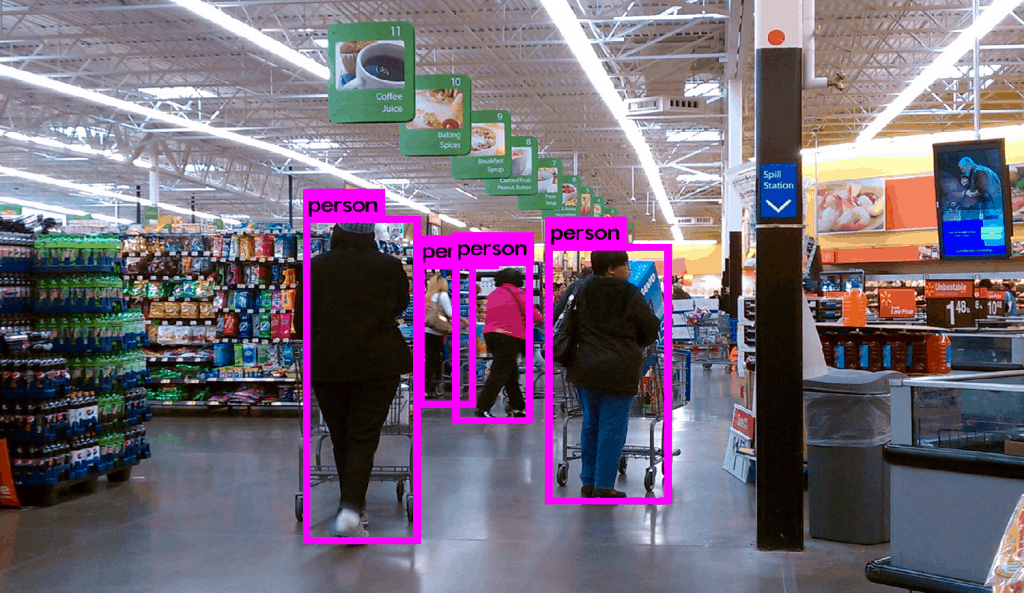
\includegraphics[scale=0.3]{graphics/supermarket.png}
  \caption{Nhận diện người đi bộ trong siêu thị}
\end{figure}

Để đạt được mục tiêu nghiên cứu, nhóm đã lựa chọn hai phương pháp để thực hiện: HOG+SVM và Faster R-CNN.

%Phương pháp HOG+SVM (Histogram of Oriented Gradients và Support Vector Machine) đã được nhóm chọn để thực nghiệm vì tính đơn giản và hiệu quả trong nhận dạng đối tượng. HOG giúp trích xuất đặc trưng từ hình ảnh bằng cách tính toán histogram các hướng cạnh trong hình ảnh. Sau đó, SVM được sử dụng để huấn luyện mô hình phân loại dựa trên các đặc trưng HOG trích xuất từ hình ảnh. Sự kết hợp của HOG và SVM cho phép chúng ta xây dựng một hệ thống nhận dạng đối tượng đơn giản và có hiệu suất tốt trong một số trường hợp.

%Ngoài ra, nhóm cũng đã chọn phương pháp Faster R-CNN (Region-based Convolutional Neural Network) để thực nghiệm do khả năng kết hợp giữa việc phân loại đối tượng và định vị vị trí chính xác của chúng. Faster R-CNN sử dụng mạng neural convolutional để trích xuất đặc trưng từ hình ảnh và sau đó sử dụng một mạng neural định vị để xác định vùng chứa các đối tượng trong hình ảnh. Phương pháp này cho phép chúng ta đạt được hiệu suất cao trong việc phát hiện và phân loại các đối tượng trong hình ảnh, đồng thời cung cấp vị trí chính xác của từng đối tượng.

%Lựa chọn hai phương pháp HOG+SVM và Faster R-CNN cho bài toán này đảm bảo một phạm vi rộng hơn trong việc so sánh và đánh giá hiệu suất của các phương pháp nhận dạng đối tượng khác nhau. Điều này giúp tăng cường kiến thức và sự hiểu biết về cách thức hoạt động và ưu điểm của từng phương pháp, từ đó đưa ra kết luận và đề xuất cho việc áp dụng trong các ứng dụng thực tế.
Việc lựa chọn hai phương pháp này xuất phát từ sự tò mò và mong muốn học hỏi thêm kiến thức về lĩnh vực thị giác máy tính. Chúng em muốn khám phá và so sánh sự khác biệt giữa các phương pháp machine learning và deep learning để hiểu rõ hơn về cách thức hoạt động và ưu điểm của từng phương pháp. Từ việc nghiên cứu này, nhóm chúng em đã được trau dồi kiến thức và hiểu biết sâu hơn về lĩnh vực đang học.

\section{Tổng quan bài toán và cơ sở lý thuyết}
%Draw pipeline%
\subsection{Bài toán}
\subsubsection{Pedestrian Detection (Nhận diện người đi bộ)}
Bài toán nhận diện người đi bộ là một bài toán trong lĩnh vực thị giác máy tính, có mục tiêu nhằm xác định và định vị vị trí của người đi bộ trong các hình ảnh hoặc video. Trong đề tài này, nhóm chỉ có khả năng nhận diện người đi bộ trong các hình ảnh. Mục tiêu của bài toán là xác định và định vị người đi bộ trong hình ảnh, cung cấp thông tin về vị trí, bounding box và lớp (như người đi bộ hay không).

Input: Một hình ảnh kỹ thuật số (hay single frame)

Output: Một hình ảnh bao gồm các tọa độ (bounding boxes) biểu thị cho vị trí của người đi bộ trong hình (nếu có).
\vfill
\graphicspath{{figures/}}
\begin{figure}[h!]
    \centering
    \subfloat[\centering Input]{{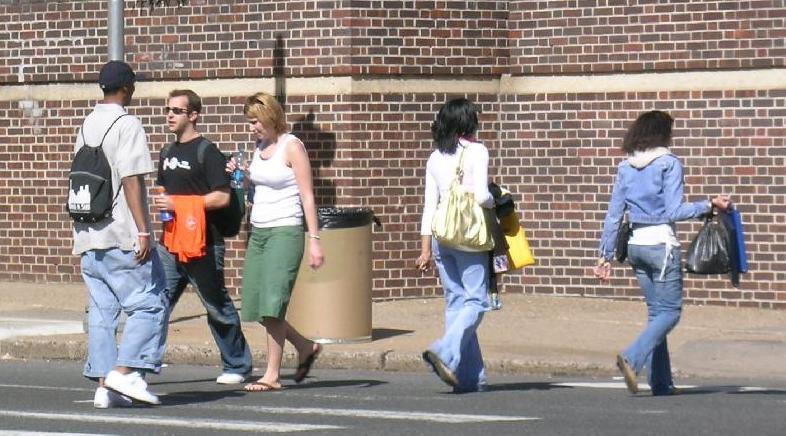
\includegraphics[width=7cm]{graphics/image_11.jpg} }}
    \qquad
    \subfloat[\centering Output]{{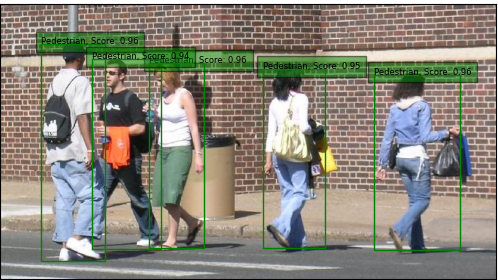
\includegraphics[width=7cm]{graphics/predicted_11.png} }}
    \caption{Một ví dụ về input và output của bài toán}
\end{figure}
\subsection{Pipeline}
Các kỹ thuật Object Detection truyền thống thường tuân theo ba bước chính được đưa ra trong hình bên dưới.

Bước đầu tiên liên quan đến việc tạo ra một số vùng đề xuất (region proposal). Từ mỗi vùng đề xuất, một vectơ đặc trưng có độ dài cố định được trích xuất bằng cách sử dụng các image descriptors khác nhau ví dụ như histogram of oriented gradients (HOG). Vector đặc trưng sau đó được sử dụng để phân loại mỗi vùng đề xuất vào lớp nền hoặc vào một trong các lớp đối tượng cụ thể. Khi số lượng lớp tăng lên, độ phức tạp của việc xây dựng một mô hình có thể phân biệt được tất cả các đối tượng này cũng tăng lên. Một trong những mô hình phổ biến được sử dụng để phân loại các vùng đề xuất là support vector machine (SVM).
\graphicspath{{figures/}}
\begin{figure}[h!]
  \centering
  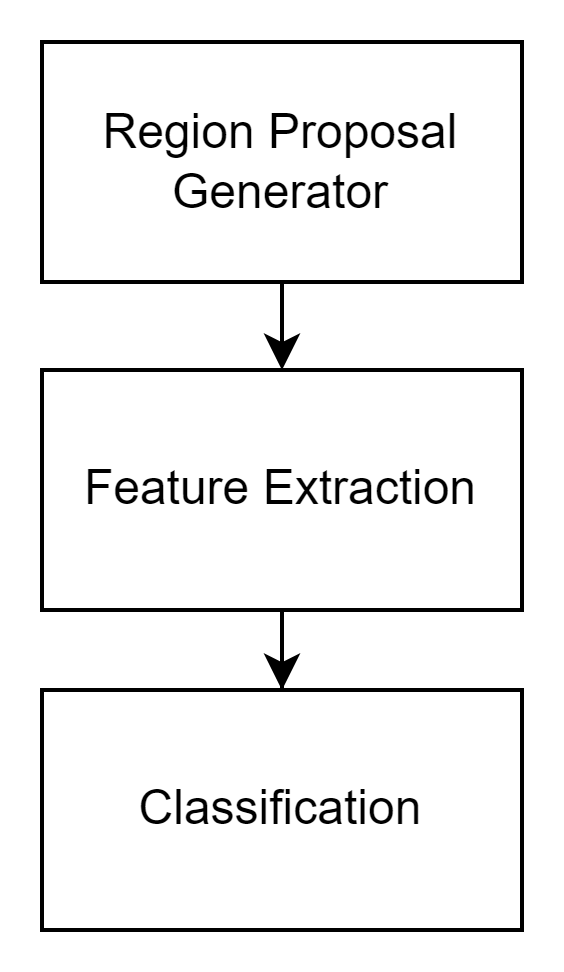
\includegraphics[scale=0.25]{graphics/pipeline.png}
  \caption{Pipeline của các phương pháp truyền thống trong Object Detection}
\end{figure}

\subsection{Độ đo}
Trong bài toán nhận dạng người đi bộ (pedestrian detection), nhóm đã sử dụng một độ đo phổ biến trong thị giác máy tính là mean Average Precision (mAP) cho việc đánh giá hiệu suất của hai phương pháp HOG+SVM và Faster R-CNN. Độ đo này được sử dụng để đánh giá độ chính xác của việc phát hiện và định vị vị trí của các người đi bộ trong hình ảnh. mAP được đo trong khoảng từ 0 đến 1.

\subsubsection{IOU}
IOU (Intersection over Union) là một phép đo sử dụng để đánh giá sự chồng chéo giữa hai khu vực được dự đoán và khu vực thực tế trong bài toán nhận dạng đối tượng. Trong bước tính mAP (mean Average Precision), IOU được sử dụng để xác định xem một đối tượng dự đoán được coi là chính xác hay không.

Để tính toán IOU, ta sử dụng hai khu vực là khu vực dự đoán (predicted region) và khu vực thực tế (ground truth region). Khu vực này được biểu diễn bằng các hình chữ nhật hoặc các đa giác đối tượng trong không gian 2D.

IOU được tính bằng cách tính tỷ lệ diện tích của khu vực giao nhau (intersection) giữa hai khu vực và diện tích của khu vực hợp nhau (union) giữa hai khu vực. Công thức tính toán IOU:
%nói về iou trước
\graphicspath{{figures/}}
\begin{figure}[h!]
  \centering
  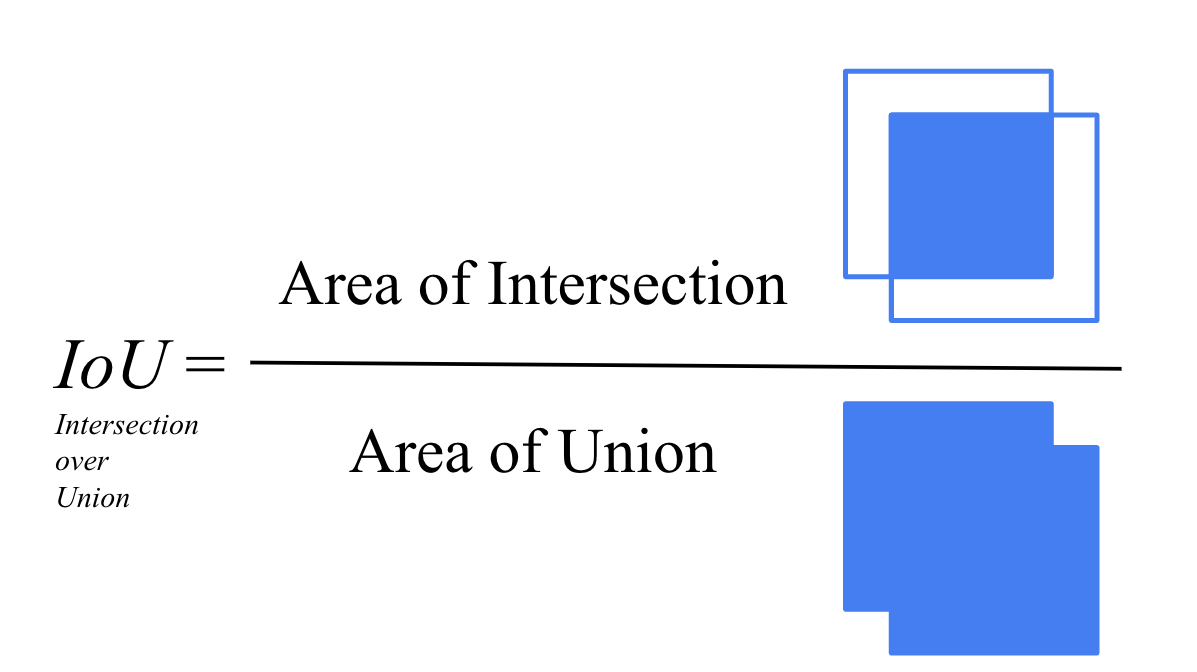
\includegraphics[scale=0.24]{graphics/iou.png}
  \caption{Cách tính IoU}
\end{figure}

Giá trị IOU nằm trong khoảng từ 0 đến 1. Nếu IOU = 0, tức là không có sự chồng chéo giữa khu vực dự đoán và khu vực thực tế. Ngược lại, nếu IOU = 1, tức là khu vực dự đoán trùng khớp hoàn toàn với khu vực thực tế.

Trong bước tính toán mAP, mỗi đối tượng dự đoán được so sánh với các đối tượng thực tế. Nếu IOU của đối tượng dự đoán với đối tượng thực tế vượt qua một ngưỡng xác định (thường là 0.5), đối tượng dự đoán được coi là chính xác. Ngược lại, nếu IOU không đạt ngưỡng này, đối tượng dự đoán được coi là sai.

\subsubsection{Confusion Matrix}
Ứng với mỗi ngưỡng xác định (IOU threshold), ta được một cặp giá trị precision và recall. Sau khi tính IOU và căn cứ vào ngưỡng xác định, ta sử dụng confusion matrix để phân tích và phân nhóm các trường hợp dự đoán của mô hình. Thông qua confusion matrix, ta có thể phân loại các trường hợp như Hình \ref{fig:confusion-matrix}.
\graphicspath{{figures/}}
\begin{figure}[h!]
  \centering
    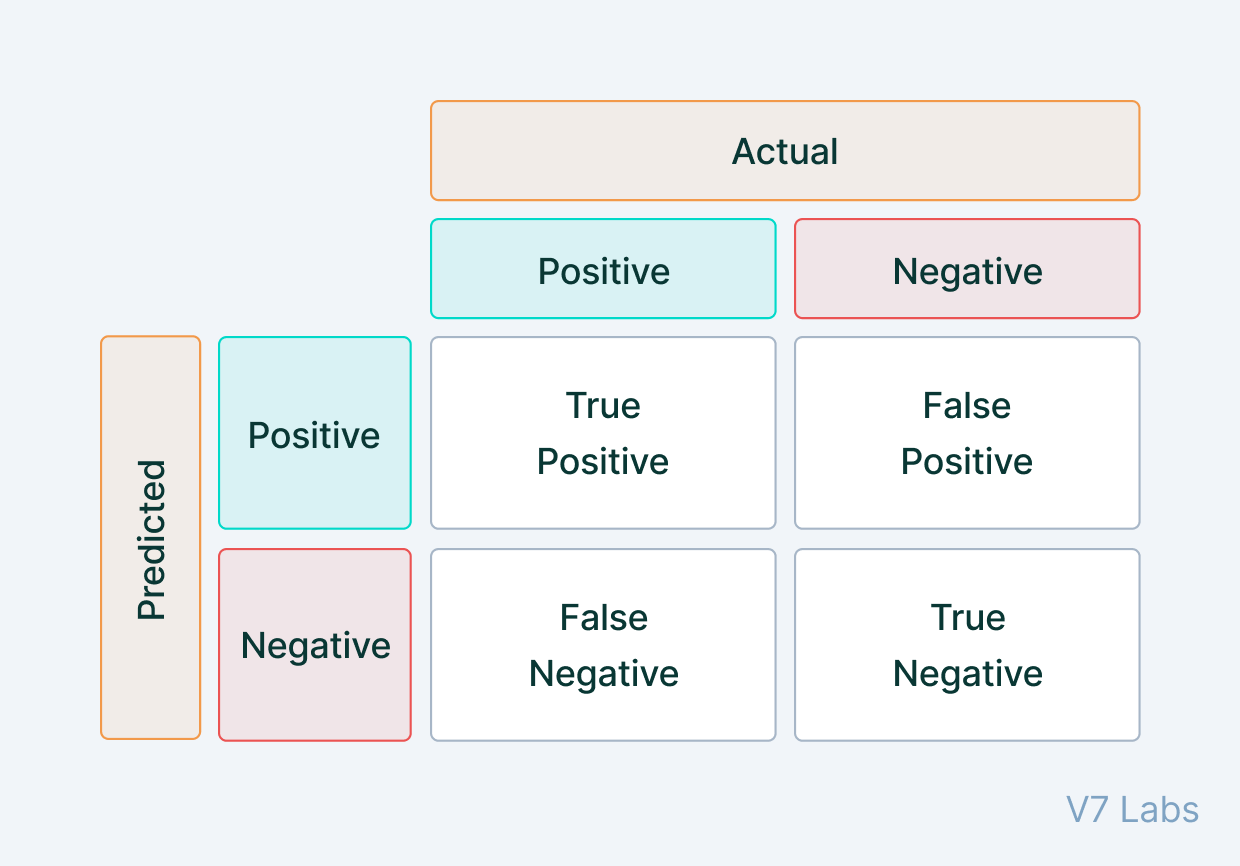
\includegraphics[scale=0.5]{graphics/confusion-matrix.png}
  \caption{Confusion matrix}
  \label{fig:confusion-matrix}
\end{figure}

\subsubsection{Tính toán mAP}
Mean Average Precision (mAP) là một độ đo tổng hợp của các giá trị Average Precision (AP) tính toán cho từng lớp (trong trường hợp này, lớp người đi bộ) trong bộ dữ liệu. Để tính toán AP, ta xây dựng đường cong Precision-Recall bằng cách thay đổi ngưỡng (threshold) phân loại và tính toán precision và recall tại mỗi ngưỡng.

Precision là tỷ lệ giữa số lượng các đối tượng được phát hiện chính xác và tổng số đối tượng được phát hiện
\begin{equation*}
    Precision = \frac{TP}{TP + FP}\nonumber
\end{equation*}
Trong khi Recall là tỷ lệ giữa số lượng các đối tượng được phát hiện chính xác và tổng số đối tượng thực tế trong hình ảnh.
\begin{equation}
    Recall = \frac{TP}{TP + FN}\nonumber
\end{equation}

Sau khi tính toán được đường cong Precision-Recall, ta tính toán giá trị AP bằng cách tính toán diện tích dưới đường cong Precision-Recall. Giá trị AP đại diện cho độ chính xác trung bình của việc phát hiện đối tượng trong các ngưỡng phân loại khác nhau. Mean Average Precision (mAP) là giá trị trung bình của AP cho tất cả các lớp (ở bài toán pedestrian detection là 1).
\begin{equation}
    mAP = \frac{|TP|}{|TP| + |FP|}\nonumber
\end{equation}
\begin{figure}[h!]
  \centering
    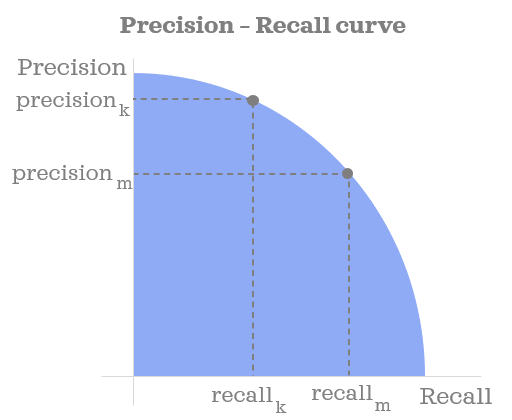
\includegraphics[scale=0.5]{graphics/curve.png}
  \caption{Đường cong Precision-Recall}
\end{figure}
Một giá trị mAP cao cho thấy hai phương pháp đều đạt được độ chính xác cao trong việc phát hiện người đi bộ trong hình ảnh. Tuy nhiên, cần lưu ý rằng mAP cũng có thể bị ảnh hưởng bởi các yếu tố khác nhau như tỉ lệ false positive (thông tin sai dương) và false negative (thông tin sai âm), độ lệch vị trí, và độ phức tạp tính toán của từng phương pháp.

Vì vậy, trong bài toán nhận dạng người đi bộ, việc so sánh mAP giữa phương pháp HOG+SVM và Faster R-CNN sẽ cung cấp thông tin quan trọng về hiệu suất và độ chính xác của cả hai phương pháp trong việc phát hiện và định vị người đi bộ trong hình ảnh.

\subsection{Các phương pháp được sử dụng trong đề tài}
\subsubsection{HOG+SVM}
\paragraph{Lý do sử dụng HOG+SVM cho bài toán\\}
Phương pháp HOG (Histogram of Oriented Gradients) kết hợp với SVM (Support Vector Machines) được chọn để giải quyết bài toán phát hiện người đi bộ với những lý do:
\begin{itemize}[noitemsep, topsep=0pt, leftmargin=1.25em, label={$-$}]
    \item Đơn giản và hiệu quả tính toán: HOG sử dụng tính toán đơn giản, nó chỉ yêu cầu tính gradient của hình ảnh và xây dựng histogram các hướng gradient. Quá trình này có thể thực hiện nhanh chóng trên các hình ảnh tĩnh và không yêu cầu tài nguyên tính toán phức tạp.
    \item Đặc trưng HOG phù hợp cho hình ảnh: HOG nhạy bén với cấu trúc dọc và đặc trưng hình học của người đi bộ, chẳng hạn như cạnh và góc cơ thể vì khả năng trích xuất thông tin hướng và độ lớn của gradient.
    \item SVM là một bộ phân loại mạnh mẽ: SVM là một thuật toán học máy được sử dụng rộng rãi trong việc phân loại và nhận dạng. SVM có khả năng tạo ra một ranh giới quyết định tối ưu giữa các lớp dữ liệu (người đi bộ và không phải người đi bộ). SVM có khả năng xử lý các bài toán phân loại tuyến tính và phi tuyến tính, điều này rất hữu ích trong việc xác định những đặc trưng phức tạp của người đi bộ trong không gian đặc trưng HOG.
    \item Độ ổn định và khả năng tổng quát hóa\cite{reasontousehogsvm}: Phương pháp HOG và SVM có khả năng ổn định và tổng quát hóa tốt đối với các biến đổi trong ánh sáng, môi trường và biến thể về cách thức di chuyển của người đi bộ. Điều này giúp cho phương pháp này có khả năng hoạt động tốt trong các tình huống thực tế.
\end{itemize}
Mặc dù hiện nay phương pháp này không được sử dụng nhiều bời các phương pháp deep learning phát triển rất mạnh mẽ nhờ khả năng học tự động và hiệu suất cao hơn của chúng, nhưng đây vẫn là một phương pháp với thuật toán đơn giản và dễ hiểu được sử dụng để giải quyết bài toán phát hiện đối tượng là người đi bộ.
\paragraph{HOG\\}
HOG (Histogram of Oriented Gradients) là một phương pháp mô tả đặc trưng dùng để biểu diễn hình dạng và diện mạo của một đối tượng trong một hình ảnh. Thuật toán HOG tính toán và biểu thị sự phân bố và hướng của gradient (độ dốc) trong hình ảnh.  

HOG được giới thiệu bởi Navneet Dalal và Bill Triggs vào năm 2005 như một phương pháp hiệu quả để phát hiện đối tượng trong ảnh, đặc biệt là trong bài toán phát hiện người đi bộ.   

Quá trình trích xuất đặc trưng HOG bao gồm các bước chính như sau:
\begin{itemize}[noitemsep, topsep=0pt, leftmargin=1.25em, label={$-$}]
    \item Chia hình ảnh thành các ô (cells): Hình ảnh được chia thành các ô nhỏ, mỗi ô đại diện cho một vùng nhỏ trên hình ảnh.
    \item Tính toán gradient: Gradient của các pixel trong mỗi ô được tính bằng cách sử dụng phương pháp gradient, để xác định độ dốc và hướng của các điểm ảnh. 
    \item Tạo histogram các hướng gradient: Dựa trên gradient, một histogram được tạo ra cho mỗi ô. Histogram này biểu thị phân bố các hướng gradient trong ô đó. 
    \item Chuẩn hóa histogram: Mỗi histogram được chuẩn hóa để giảm ảnh hưởng của ánh sáng và độ tương phản. Thông thường, chuẩn hóa được thực hiện bằng cách chuẩn hóa L2 (Euclidean) của histogram, tức là chuẩn hóa tổng bình phương các giá trị trong histogram về 1.
    \item Kết hợp các vector đặc trưng HOG: Các vector đặc trưng HOG của các ô liền kề được kết hợp thành một vector đặc trưng duy nhất cho toàn bộ hình ảnh. Bước này giúp bao gồm thông tin về sự phân bố của đặc trưng trên cả hình ảnh.
\end{itemize}
\pagebreak
\begin{figure}[h!]
  \centering
  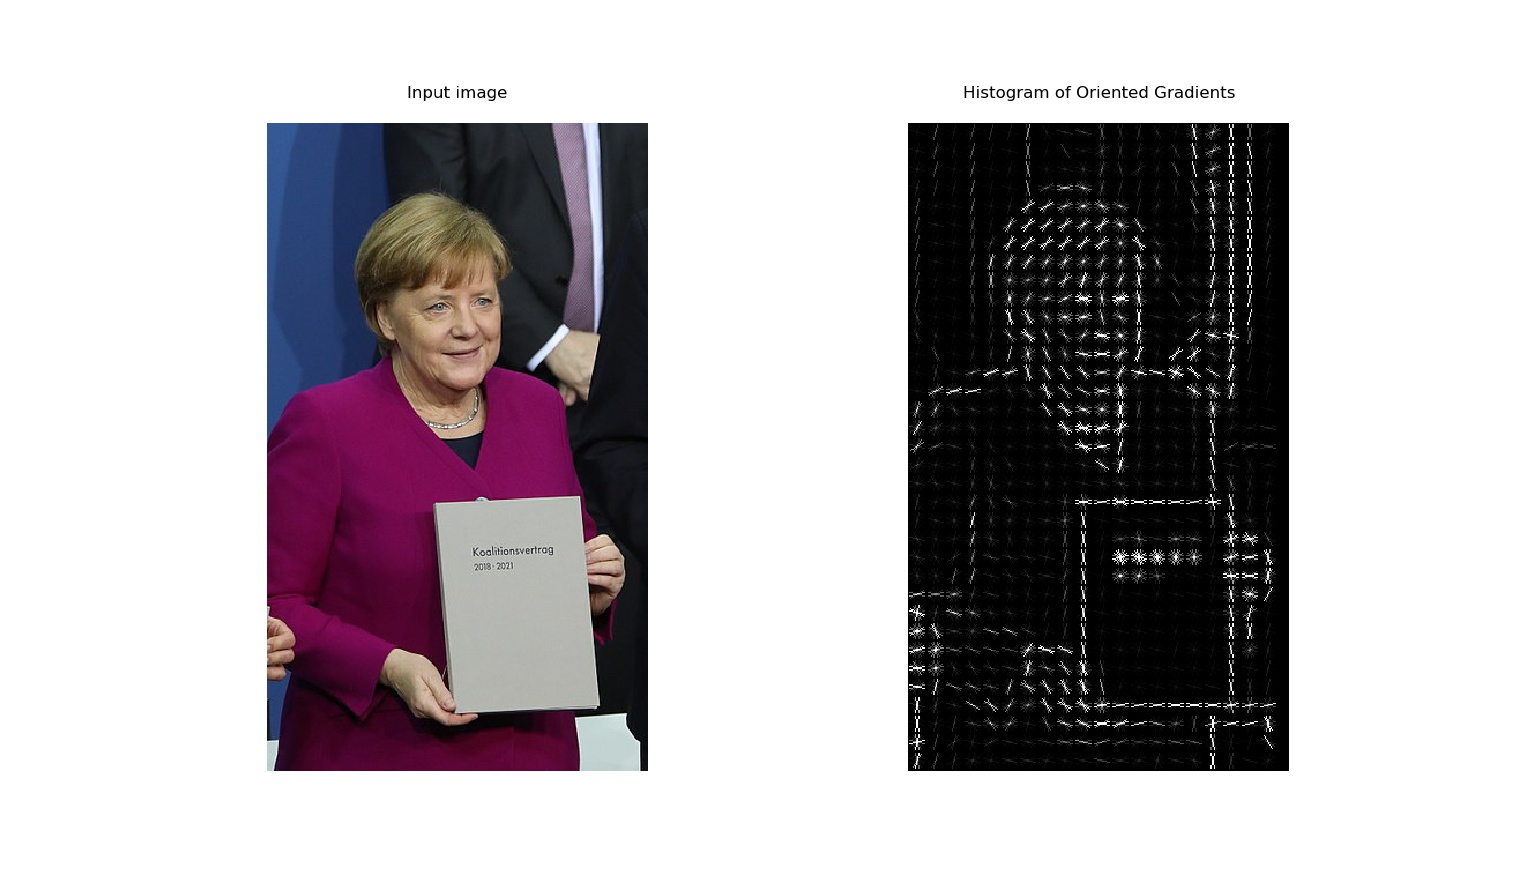
\includegraphics[scale=0.35]{graphics/HOG.jpeg}
  \caption{Kết quả của quá trình trích xuất đặc trưng HOG}
\end{figure}

\paragraph{SVM\\}
Support Vector Machine là một thuật toán máy học có giám sát, sử dụng để phân loại và dự báo. Trong việc phát hiện đối tượng, SVM thường được sử dụng như một bộ phân loại để phân biệt giữa đối tượng cần phát hiện và nền.

SVM hoạt động bằng cách tìm ra siêu phẳng tối ưu (hyper-plane) để phân tách các điểm dữ liệu vào các lớp khác nhau. Nó cố gắng tối ưu hóa khoảng cách giữa hyper-plane và các điểm dữ liệu gần nhất của mỗi lớp. Các điểm dữ liệu nằm trên ranh giới hoặc trong ranh giới được gọi là các vector hỗ trợ (support vectors). SVM có thể xử lý dữ liệu không tách biệt tuyến tính bằng cách sử dụng hàm kernel để biến đổi không gian đầu vào thành không gian đặc trưng có số chiều cao hơn.
\graphicspath{{figures/}}
\begin{figure}[h!]
  \centering
  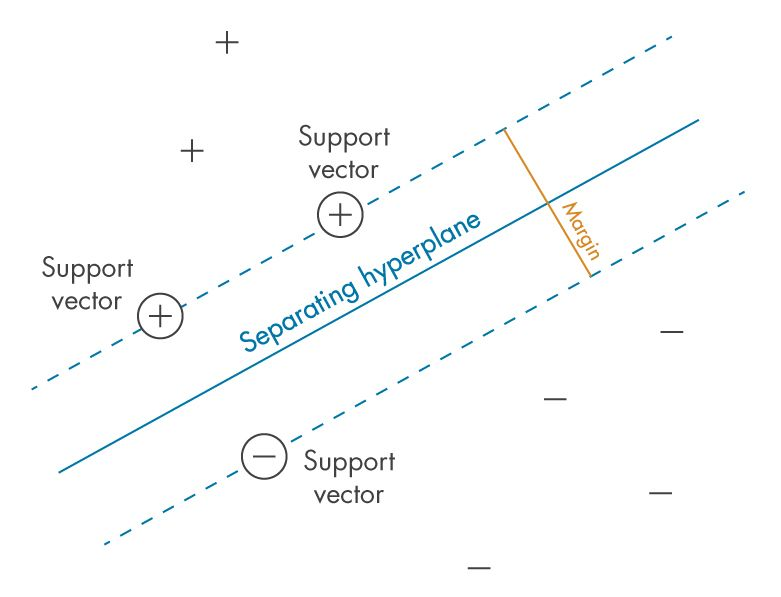
\includegraphics[scale=0.35]{graphics/SVM.jpg}
  \caption{SVM tối ưu hóa khoảng cách giữa hyper-plane và các support vector}
\end{figure}

Các bước chính trong quá trình huấn luyện SVM là:
\begin{itemize}[noitemsep, topsep=0pt, leftmargin=1.25em, label={$-$}]
    \item Xác định đặc trưng: Dữ liệu đầu vào cần được biểu diễn bằng các đặc trưng có ý nghĩa. Các đặc trưng này thường được trích xuất thông qua các phương pháp như HOG, SIFT.
    \item Xây dựng mô hình: Sau khi có các đặc trưng, mô hình SVM được xây dựng bằng việc tìm ra siêu phẳng tốt nhất để phân tách các lớp dữ liệu. Có nhiều loại SVM khác nhau như SVM tuyến tính, SVM hạt nhân (kernel SVM) và SVM đa lớp (multiclass SVM).
    \item Tối ưu hóa: Mục tiêu của SVM là tìm ra hyper-plane tối ưu sao cho khoảng cách (margin) từ siêu phẳng đến các support vectors là lớn nhất. Quá trình này thường được thực hiện bằng cách giải một bài toán tối ưu hóa bậc hai.
    \graphicspath{{figures/}}
    \begin{figure}[h!]
      \centering
      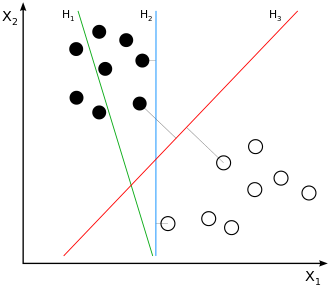
\includegraphics[scale=0.6]{graphics/Svm_separating_hyperplanes.png}
      \caption{H3 là hyper-plane tối ưu với margin tối đa ngăn cách các support vectors}
    \end{figure}
    \item Dự đoán: Sau khi huấn luyện mô hình, SVM có thể được sử dụng để dự đoán lớp của các điểm dữ liệu mới dựa trên vị trí của chúng đối với hyper-plane đã xác định.
\end{itemize}    
Support Vector Machine hiểu một cách đơn giản là một biên giới để chia hai lớp tốt nhất. Đây là một thuật toán học máy mạnh mẽ và đa dụng, một phương pháp hiệu quả cho bài toán phân lớp dữ liệu. SVM cũng có khả năng phân loại tốt trên các tập dữ liệu lớn và ít bị ảnh hưởng bởi nhiễu. Tuy nhiên, nó cũng đòi hỏi tính toán phức tạp và lựa chọn tham số cho phù hợp. Quá trình huấn luyện SVM có thể yêu cầu nhiều tài nguyên tính toán và thời gian, đặc biệt là trên các tập dữ liệu lớn. SVM có các tham số như hàm kernel, thông số đường mềm (soft margin), và hệ số điều chỉnh. Lựa chọn tham số đúng cũng là một yếu tố quan trọng để đạt được hiệu suất tốt của mô hình SVM.
\subsubsection{Faster R-CNN}
Trước khi đi vào Faster R-CNN, ở báo cáo này nhóm sẽ giới thiệu sơ lược về các mô hình cùng thuộc gia đình R-CNN trong bài toán object detection bao gồm: R-CNN, Fast R-CNN.

\paragraph{R-CNN (Region with CNN feature)\\}

R-CNN \cite{rcnn} là một thuật toán two-stage để phát hiện vật thể. Ý tưởng của bài toán R-CNN khá đơn giản:
\begin{itemize}[noitemsep, topsep=0pt, leftmargin=1.25em, label={$-$}]
    \item Bước 1: Dùng thuật toán Selective Search để lấy ra khoảng 2000 bounding box trong input mà có khả năng chứa đối tượng.
    \item Bước 2: Với mỗi vùng bounding box ta xác định nó là đối tượng nào.
\end{itemize}

Nói về thuật toán Selective Search thì đây là thuật toán đề xuất khu vực cho các công việc Object Detection. Nó chia ảnh thành các phần với với mật độ điểm ảnh dựa trên phương pháp phân đoạn dựa trên đồ thị của Felzenszwalb và Huttenlocher.Sau đó, Selective Search sử dụng các phần đã chia được và thực hiện các bước sau:
\begin{enumerate}[topsep=0pt,itemsep=-1ex,partopsep=1ex,parsep=1ex]
    \item Thêm các bounding box tương ứng với phần đã được phân đoạn vào danh sách các region proposals (vùng đề xuất)
    \item Nhóm các phân đoạn liền kề dựa trên sự tương đồng
    \item Quay lại bước 1
\end{enumerate}

Tại mỗi lần lặp lại, các phân đoạn lớn hơn được hình thành và thêm vào danh sách các region proposals.

\begin{figure}[h!]
  \centering
  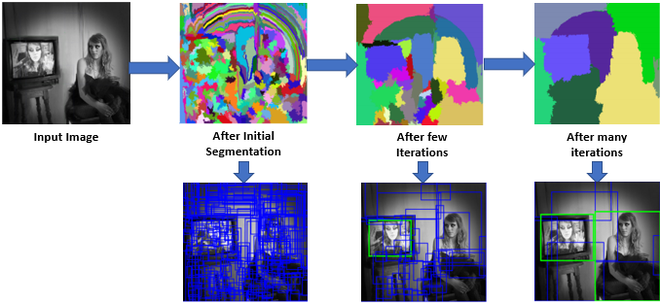
\includegraphics[scale=0.58]{graphics/selective search.png}
  \caption{Sử dụng Selective Search để tạo ra các bounding box}
\end{figure}

Kiến trúc của R-CNN gồm 3 thành phần:
\begin{itemize}[noitemsep, topsep=0pt, leftmargin=1.25em, label={$-$}]
    \item Vùng đề xuất hình ảnh: có tác dụng tạo và trích xuất các vùng đề xuất chứa vật thể được bao bởi các bounding box. 
    \item Trích xuất đặc trưng (feature extractor): trích xuất các đặc trưng giúp nhận diện hình ảnh từ các region proposals thông qua các mạng convolutional neural network (CNN).
    \item Phân loại (classifier): dựa vào input là các features ở phần trước để phân loại hình ảnh chứa trong region proposal về đúng nhãn.
\end{itemize}
\graphicspath{{figures/}}
\begin{figure}[h!]
  \centering
  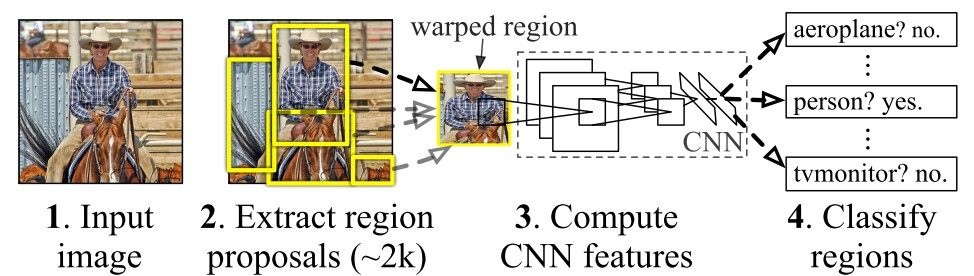
\includegraphics[scale=0.45]{graphics/RCNN.jpg}
  \caption{Sơ đồ pipeline xử lý trong mô hình R-CNN}
\end{figure}

Một trong những cải tiến của R-CNN là sử dụng mô hình SVM (Support Vector Machine) để phân loại các vùng đề xuất và mô hình hồi quy (bounding box regression) riêng biệt để dự đoán vị trí. Qua đó, mô hình R-CNN có khả năng đạt được kết quả chính xác trong việc nhận diện và định vị vật thể trong ảnh.\\
Tuy R-CNN đạt được kết quả khá tốt trong bài toán Object Detection, tuy nhiên, quá trình huấn luyện và dự đoán của mô hình này khá chậm do cần phải xử lý mỗi region proposal một cách độc lập như ở hình trên cần phải xử lý khoảng 2000 vùng đề xuất cho mỗi hình ảnh tại thời điểm thử nghiệm.

\paragraph{Fast R-CNN\\}
Dựa trên thành công của R-CNN, Ross Girshick (lúc này đã chuyển sang Microsoft Research) và các cộng sự của ông đã đề xuất một phương pháp mở rộng để giải quyết các hạn chế của R-CNN trong một bài báo vào năm 2015 với tiêu đề ngắn gọn là Fast R-CNN \cite{fastrcnn}.

Trong bài báo, nhóm tác giả đã chỉ ra những hạn chế của R-CNN đó là:
\begin{itemize}[noitemsep, topsep=0pt, leftmargin=1.25em, label={$-$}]
    \item Quá trình huấn luyện qua một pipeline phức tạp: R-CNN yêu cầu một pipeline gồm nhiều bước, bao gồm chuẩn bị dữ liệu, huấn luyện mạng CNN và các mô hình phụ trợ như SVM. Quá trình này phức tạp và tốn nhiều thời gian và công sức.
    \item Chi phí training tốn kém về số lượng bounding box và thời gian huấn luyện: R-CNN đòi hỏi huấn luyện mạng CNN trên một lượng lớn region proposal cho mỗi hình ảnh. Điều này dẫn đến việc tốn kém về tài nguyên tính toán và thời gian huấn luyện.
    \item Phát hiện đối tượng chậm: Do quá trình phải xử lý một lượng lớn region proposal, R-CNN không đảm bảo tốc độ phát hiện vật thể trong thời gian thực (real-time).
\end{itemize}
\graphicspath{{figures/}}
\begin{figure}[h!]
  \centering
  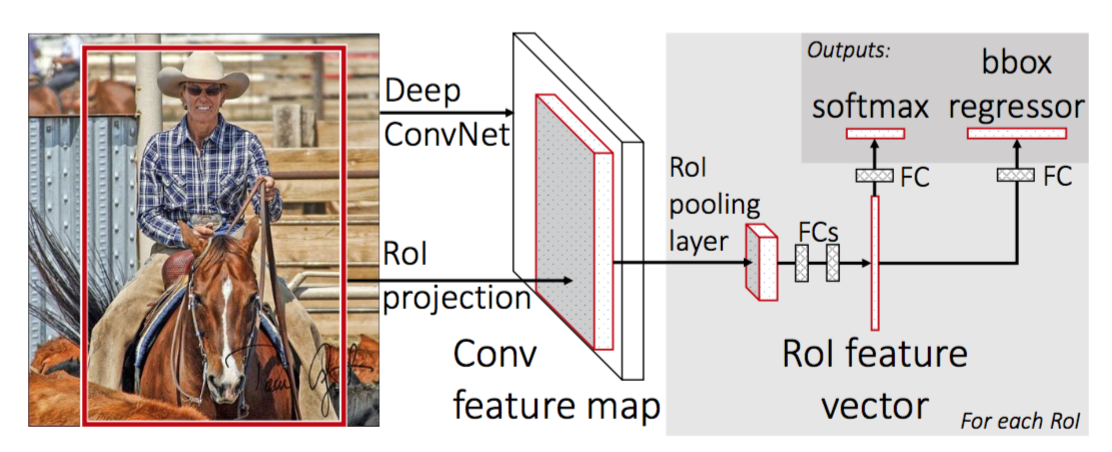
\includegraphics[scale=0.35]{graphics/fast-RCNN.png}
  \caption{Sơ đồ pipeline xử lý trong mô hình Fast R-CNN}
\end{figure}
Cách tiếp cận của mô hình Fast R-CNN khá giống với R-CNN tuy nhiên, thay vì đưa các vùng đề xuất (region proposals) qua mạng CNN, Fast R-CNN đưa hình ảnh đầu vào qua một mạng CNN duy nhất để trích xuất ra được convolutional feature map. Điều này giúp tái sử dụng đặc trưng cho toàn bộ ảnh và giảm thiểu thời gian tính toán so với R-CNN. Từ convolution feature map, Fast R-CNN sử dụng kỹ thuật RoI Pooling để chuyển đổi các vùng đề xuất có kích thước và hình dạng khác nhau thành các vùng có kích thước cố định. Sau đó, các vùng này được đưa qua các lớp Fully-Connected để phân loại và dự đoán vị trí. Cuối cùng mô hình chia thành hai đầu ra, một đầu ra cho dự đoán nhãn thông qua một softmax layer và một đầu ra khác dự đoán bounding box (kí hiệu là bbox) dựa trên hồi qui tuyến tính. Quá trình này sau đó được lặp lại nhiều lần cho mỗi vùng RoI trong một hình ảnh.

Ở trên, ta có đề cập tới một thuật ngữ là RoI Pooling. Region of Interest (RoI) pooling là một dạng của pooling layer. Điểm khác so với max pooling hay average pooling là bất kể kích thước của tensor input, RoI pooling luôn cho ra output có kích thước cố định được định nghĩa trước. Nó được sử dụng để biến đổi vùng đề xuất có kích thước khác nhau thành các vùng đặc trưng có kích thước cố định, giúp thuận tiện cho việc sử dụng các mạng nơ-ron fully connected.

Giả sử input của RoI pooling có kích thước m*n, trong đó m là chiều cao và n là chiều rộng của vùng đề xuất. Output của ROI pooling có kích thước h*k, với h và k thường được chọn nhỏ, ví dụ như 7*7.

Cách thức hoạt động của RoI pooling như sau:
\begin{enumerate}[topsep=0pt,itemsep=-1ex,partopsep=1ex,parsep=1ex]
    \item Chia vùng đề xuất thành h x k ô con có kích thước gần bằng nhau. Số ô con hình thành từ việc chia này sẽ bằng h*k.
    \item Đối với mỗi ô con, tìm giá trị tối đa (max pooling) từ vùng tương ứng trên input.
    \item Gom các giá trị tối đa này thành một vectơ đặc trưng có kích thước h*k.
\end{enumerate}

Qua quá trình này, RoI pooling thu được các vùng đặc trưng có kích thước cố định h*k, không phụ thuộc vào kích thước ban đầu của vùng đề xuất.

Sự khác biệt giữa Fast R-CNN và R-CNN là ở cách thức thực hiện feature map và tính toán trên region proposals. Trong Fast R-CNN, feature map được tạo từ cả ảnh đầu vào, và sau đó các region proposals được trích xuất từ feature map. Trái lại, R-CNN tách riêng các region proposal và thực hiện CNN trên từng region proposal.

\graphicspath{{figures/}}
\begin{figure}[h!]
  \centering
  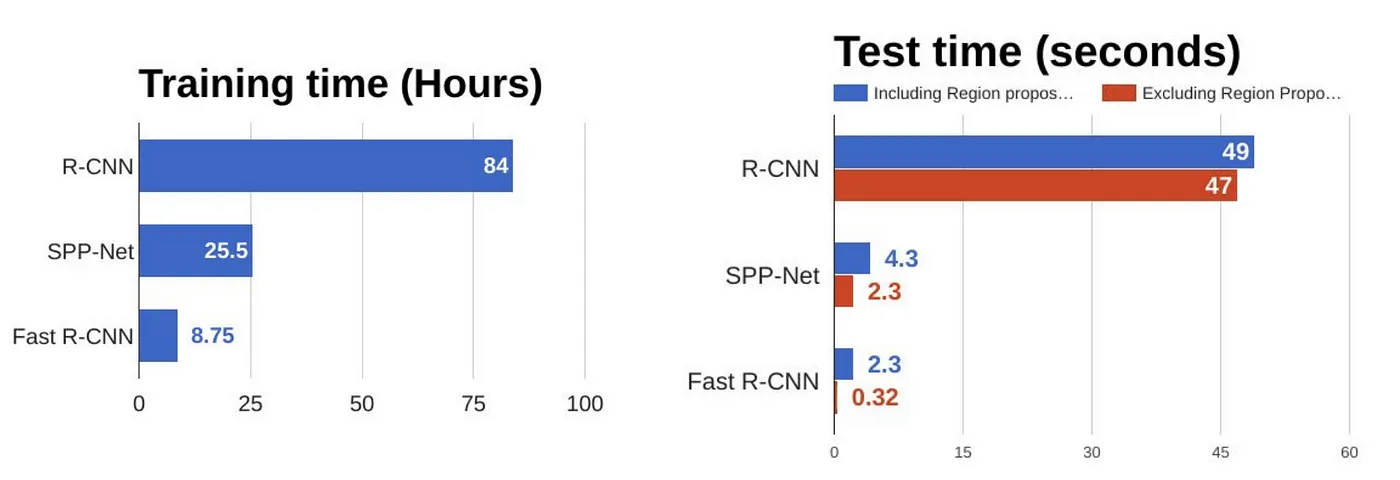
\includegraphics[scale=0.3]{graphics/Fast R-CNN compare.png}
  \caption{Biểu đồ so sánh thời gian giữa R-CNN, SPP-Net và Fast R-CNN \cite{compare}}
\end{figure}

Dựa vào hình trên, ta có thể thấy rằng Fast R-CNN mang lại kết quả tốt, với hiệu suất vượt trội so với R-CNN trong quá trình huấn luyện và thực nghiệm. Khi xem xét hiệu suất của Fast R-CNN trong thời gian thực nghiệm, việc bao gồm các vùng đề xuất làm chậm thuật toán một cách đáng kể so với việc không sử dụng các vùng đề xuất. Do đó, vùng đề xuất trở thành bottleneck trong mô hình Fast R-CNN, ảnh hưởng đến hiệu suất của nó.

\paragraph{Faster R-CNN\\}
Kiến trúc mô hình đã được cải thiện hơn nữa về cả tốc độ huấn luyện và phát hiện được đề xuất bởi Shaoqing Ren và các cộng sự tại Microsoft Research trong bài báo năm 2016 có tiêu đề Faster R-CNN: Towards Real-Time Object Detection with Region Proposal Networks \cite{fastercnn}. Dịch nghĩa là “Faster R-CNN: Hướng tới phát hiện đối tượng theo thời gian thực với các mạng đề xuất khu vực”.

Mặc dù Faster R-CNN là một mô hình đơn lẻ duy nhất nhưng nó kết hợp 2 modules:
\begin{itemize}[noitemsep, topsep=0pt, leftmargin=1.25em, label={$-$}]
    \item Mạng đề xuất khu vực (Region Proposal Network): Mạng CNN để đề xuất các vùng và loại đối tượng cần xem xét trong vùng
    \item Fast R-CNN: Mạng CNN để trích xuất các features từ các region proposal và trả ra các bounding box và nhãn
\end{itemize}

\subparagraph{Region Proposal Network (RPN)\\}
Faster R-CNN không dùng thuật toán Selective Search để lấy ra các region proposal, mà nó thêm một mạng CNN mới mà trong bài báo trên tác giả gọi là Region Proposal Network (RPN) để tìm các region proposal.

\graphicspath{{figures/}}
\begin{figure}[h!]
  \centering
  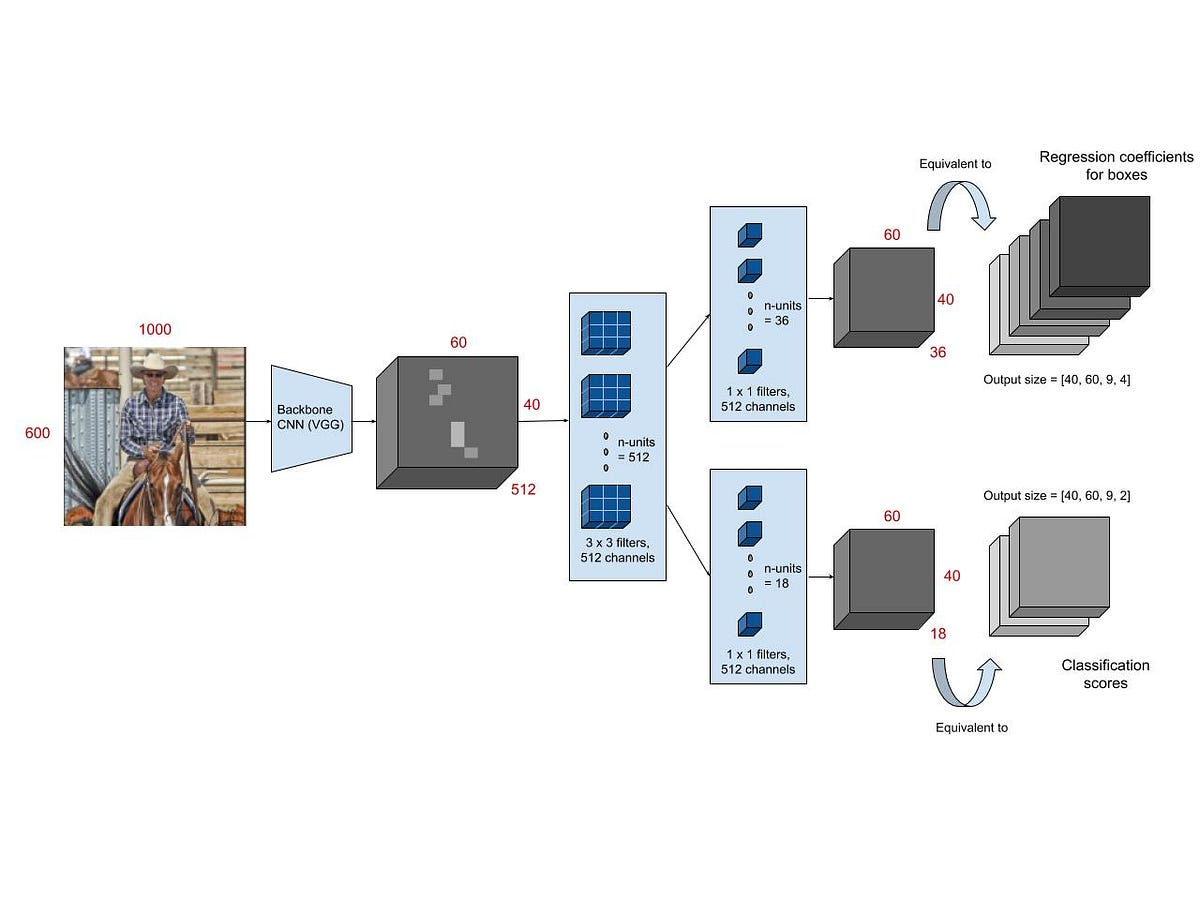
\includegraphics[scale=0.3]{graphics/rpn.jpg}
  \caption{Cấu trúc của Region Proposal Networks (RPN)}
\end{figure}

Về cơ bản thì ta có thể thấy rằng mô hình Faster RCNN kế thừa từ Fast RCNN bằng việc thay Selective Search bằng lớp RPN. 
RPN bắt đầu bằng việc đưa hình ảnh đầu vào vào backbone convolutional neural network. Ảnh đầu vào được thay đổi kích thước sao cho chiều rộng ngắn nhất là 600px và chiều dài không vượt quá 1000px.

Đầu ra của backbone network là một feature map thường nhỏ hơn nhiều so với ảnh đầu vào tùy thuộc vào bước đi (stride) của backbone network, nhưng vẫn giữ lại thông tin về các đặc trưng quan trọng của ảnh. Đối với hai backbone network được sử dụng trong bài báo (VGG, ZF-Net), bước đi của mạng là 16. Điều này có nghĩa là hai điểm liên tiếp trong đặc trưng đầu ra của backbone network tương ứng với hai điểm cách nhau 16 pixels trên ảnh đầu vào.

Trên feature map, RPN sử dụng một cửa sổ trượt (sliding window) có kích thước cố định để duyệt qua từng vị trí trên feature map. Tại mỗi vị trí, RPN áp dụng một số anchors, có thể hiểu là các pre-defined boxes được định nghĩa trước lúc khi huấn luyện mô hình, để dự đoán xem vùng đó có chứa vật thể hay không và điều chỉnh kích thước của anchors để chính xác phù hợp với vật thể. Hình dưới đây cho thấy 9 anchor có tỷ lệ khía cạnh và kích thước khác nhau được đặt trên ảnh đầu vào cho một điểm pixel A trên bản đồ đặc trưng (feature map) đầu ra. Đối với bộ dữ liệu PASCAL, các anchor được sử dụng có 3 tỷ lệ kích thước là \(128^2\), \(2256^2\), \(512^2\) và 3 tỷ lệ khía cạnh là 1:1, 1:2 và 2:1.
\graphicspath{{figures/}}
\begin{figure}[h!]
  \centering
  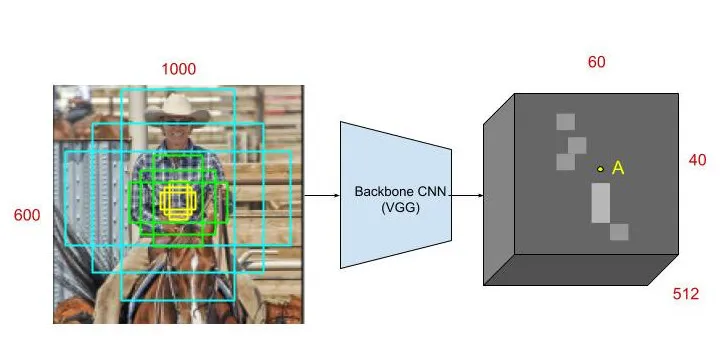
\includegraphics[scale=0.45]{graphics/anchor.png}
  \caption{Các anchors có thể có trong hình ảnh đầu vào ở một vị trí tương ứng với điểm A trong feature map}
\end{figure}

Các anchor thông thường được định nghĩa với 3 anchor size và 3 anchor ratio khác nhau và do đó có tổng cộng k = 9 anchor (k cũng có thể khác 9). Ví dụ feature map đầu ra đang là 37x50x256 thì tổng số anchor box sẽ là 37x50x9=16650. Các anchor box được đưa vào thuật toán NMS để chắc chắn rằng các vùng dự đoán không chồng chéo lên nhau. Kết thúc RPN sẽ được đưa vào lớp RoI Pooling (đã đề cập ở Fast R-CNN) để cố định kích thước đầu vào các feature map trước khi đưa vào mạng gồm nhánh fully connected.

Các anchor này được gán cho các nhãn là positive hoặc negative (object hoặc background) dựa vào diện tích trùng lặp hay IoU (đã đề cập ở phần độ đo) với ground-truth bounding box theo quy tắc sau:
\begin{itemize}[noitemsep, topsep=0pt, leftmargin=1.25em, label={$-$}]
    \item Các anchor có tỉ lệ IoU lớn nhất với ground-truth box sẽ được coi là positive
    \item Các anchor có tỉ lệ IoU \(\geq 0.7\) sẽ được coi là positive
    \item Các anchor có tỉ lệ IoU < 0.3 sẽ được coi là negative (background)
    \item Các anchor nằm trong khoảng \(0.3 \leq x < 0.7\) sẽ được coi là neutral (trung tính) là sẽ không được sử dụng trong quá trình huấn luyện mô hình
\end{itemize}
\graphicspath{{figures/}}
\begin{figure}[h!]
  \centering
  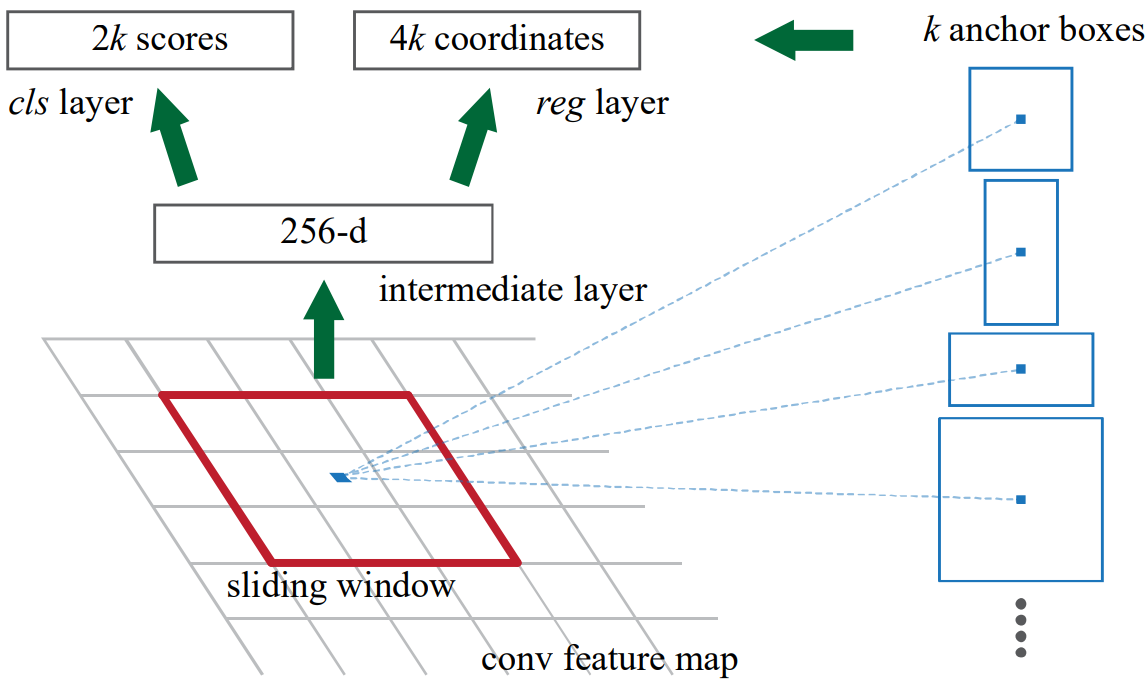
\includegraphics[scale=0.45]{graphics/rpn.png}
  \caption{Region Proposal Network (RPN)}
\end{figure}

Với mỗi vùng đề xuất kích thước nxn, một vector đặc trưng (có độ dài 256 với ZF net và 512 với VGG-16 net) được trích xuất. Vector này được đưa qua 2 lớp mạng fully connected:
\begin{enumerate}[topsep=0pt,itemsep=-1ex,partopsep=1ex,parsep=1ex]
    \item Lớp fully connected (FC) đầu tiên được gọi là "cls" đóng vai trò là một bộ phân loại nhị phân. Nó dùng để tính độ tin cậy (objectness score) cho mỗi region proposal, tức là xác định xem vùng đó có chứa đối tượng hay chỉ là phần nền (background).
    \item Lớp FC thứ hai được gọi là "reg" và trả về một vector 4 chiều, xác định các tọa độ bounding box của region proposal. Vector này cung cấp thông tin về vị trí và kích thước của đối tượng trong vùng đề xuất.
\end{enumerate}
Với binary object classification sẽ cho đầu ra là 2k channel output với k ở đây là tổng số lượng anchor box với 2 ở đây là vì chúng ta chỉ quan tâm box đó có chưa đối tượng hay không. Với bounding box regression thì có 4k channel output, với 4 là đặc trưng cho 4 tọa độ offset (x, y, w, h). 

\subparagraph{Hàm loss\\}
Trong paper thì tác giả có sử dụng hàm smooth-L1 loss, hàm loss của RPN là loss tổng của classification và regression.
\begin{equation*}
    L({p_i}, {t_i}) = \frac{1}{N_{cls}}\sum_i L_{cls}(p_i, p^*_i) + \lambda \frac{1}{N_{reg}}\sum_i p^*_i L_{reg}(t_i, t^*_i)
\end{equation*}
Trong đó:
\begin{itemize}[noitemsep, topsep=0pt, leftmargin=1.25em, label={$-$}]
    \item i là chỉ số của một anchor trong một mini-batch và \(p_i\) là xác suất dự đoán của anchor i là một đối tượng.
    \item \(p^*_i\) có giá trị 1 nếu anchor là positive (chứa đối tượng), và có giá trị 0 nếu anchor là negative (không chứa đối tượng).
    \item \(t_i\) là một vector biểu diễn 4 thông số của bounding box dự đoán
    \item \(t^*_i\) là vector tương ứng với ground-truth box của positive anchor
    \item \(L_{cls}\) là mất mát log trên hai lớp (đối tượng và không đối tượng)
    \item \(L_{reg}(t_i, t^*_i) = R(t_i - t^*_i)\), trong đó R là hàm mất mát robust (smooth L1)
    \item \(\lambda\) là một tham số cân bằng (mặc định $\lambda = 10$)
\end{itemize}
Các đầu ra của các lớp cls và reg bao gồm $p_i$ và $t_i$ tương ứng.

Đối với các bounding box hồi quy, tác giả đã tham số hóa 4 biến $t_x, t_y, t_w, t_h$ và được tính như sau:
\begin{gather*}
    t_x = (x - x_a)/w_a,\ t_y = (y - y_a)/h_a,\\
    t_w = log(w/w_a)/w_a,\ t_h = (h/h_a),\\
    t^*_x = (x^* - x_a)/w_a,\ t*_y = (y^* - y_a)/h_a,\\
    t^*_w = log(w^*/w_a)/w_a,\ t*_h = (h^*/h_a)
\end{gather*}

Các biến x, $x_a$, $x^*$ lần lượt là predicted box, anchor box, và ground-truth box (tương tự với y, w và h)

\subparagraph{Faster R-CNN (RPN + Fast RCNN)\\}
Như đã giới thiệu ở trên thì kiến trúc của Faster R-CNN bao gồm RPN dưới dạng thuật toán đề xuất khu vực và Fast R-CNN dưới dạng detector network.

\graphicspath{{figures/}}
\begin{figure}[h!]
  \centering
  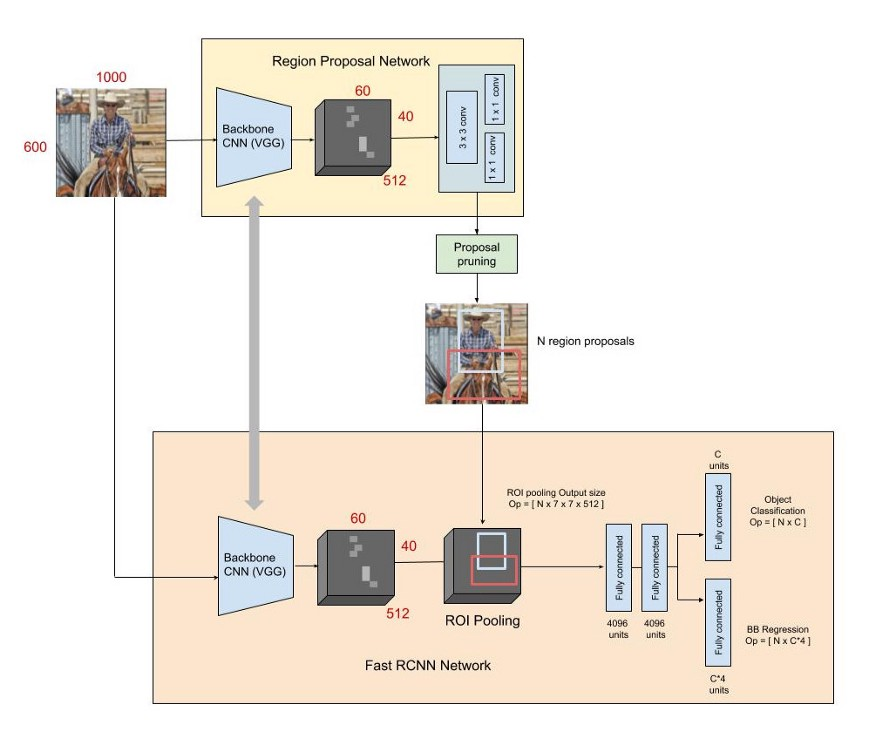
\includegraphics[scale=0.42]{graphics/fasterrcnn.jpeg}
  \caption{RPN cho các đề xuất khu vực và Fast R-CNN dưới dạng detector trong Faster R-CNN pipeline}
\end{figure}

Fast R-CNN cũng bao gồm một mạng CNN cơ bản, một lớp RoI pooling và các lớp fully connected được theo sau bởi hai nhánh đồng cấu trúc để thực hiện phân loại và hồi quy các bounding box.

Ảnh đầu vào trước tiên được truyền qua mạng CNN cơ bản để có trích xuất ra được feature map (Kích thước đặc trưng: 60, 40, 512). Bên cạch hiệu quả về thời gian thử nghiệm, một lý do quan trọng khác để sử dụng RPN như một công cụ tạo các vùng đề xuất là lợi ích của việc chia sẻ trọng số giữa mạng CNN của RPN và mạng CNN của Fast R-CNN.
Tiếp theo, các bounding box đề xuất từ RPN được sử dụng để tạo các đặc trưng từ feature map. Điều này được thực hiện bằng lớp RoI pooling. Lớp RoI pooling hoạt động bằng cách: Lấy vùng tương ứng với một đề xuất từ feature map; b) Chia vùng này thành một số cửa sổ con cố định; c) Thực hiện max-pooling trên các cửa sổ con này để tạo ra đầu ra có kích thước cố định.
Đầu ra từ lớp RoI pooling có kích thước (N, 7, 7, 512) trong đó N là số vùng đề xuất từ RPN. Sau khi chạy qua hai lớp fully connected, các đặc trưng được đưa vào các classification layer và regression layer.

Lưu ý rằng các nhánh classification và regression này khác với nhánh của RPN. Ở đây, classification layer có C đơn vị cho mỗi lớp trong mỗi lần phát hiện (bao gồm lớp background). Các đặc trưng được truyền qua lớp softmax để có được classification scores - xác suất của một vùng đề xuất thuộc về từng lớp. Các hệ số của regression layer được sử dụng để cải thiện việc dự đoán các bounding box. Ở đây, regression layer không phụ thuộc vào kích thước (không giống với RPN), nhưng phụ thuộc vào từng lớp. Điều đó có nghĩa là tất cả các lớp đều có regression layer riêng với 4 tham số mỗi lớp tương ứng với C*4 đơn vị đầu ra trong regression layer.

\paragraph{Lý do sử dụng Faster R-CNN cho bài toántoán\\}

Sau khi tìm hiểu về các mô hình như nhóm đã trình bày thì việc chọn Faster R-CNN làm mô hình để thực nghiệm cho bài toán nhận diện người đi bộ là một quyết định có cơ sở và hy vọng mang lại kết quả tốt trong việc giám sát và phân loại người đi bộ trong các môi trường thực tế. Từ biểu đồ sau đây, ta có thể thấy rằng, Faster R-CNN có hiệu suất tốt hơn rất nhiều so với các mô hình khác trong gia đình R-CNN. Đó cũng chính là lý do vì sao nhóm chọn mô hình này để thực nghiệm và đánh giá. 

\begin{figure}[h!]
  \centering
  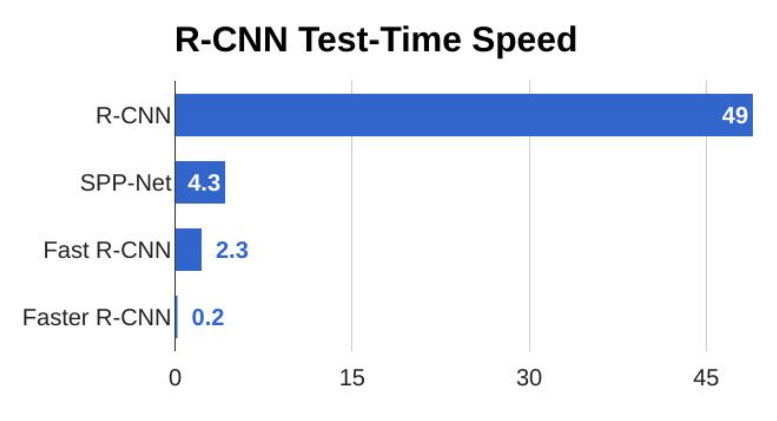
\includegraphics[scale=0.6]{graphics/whychoosefaster.png}
  \caption{Biểu đồ đánh giá về thời gian thực nghiệm của các mô hình họ R-CNN \cite{slide}}
\end{figure}



\section{Thực nghiệm}
\subsection{Môi trường}
Nhóm đã sử dụng môi trường Google Colaboratory để thực hiện nghiên cứu và phát triển trong bài toán nhận diện người đi bộ. Google Colaboratory (hay gọi tắt là Colab) là một môi trường máy tính trong đám mây miễn phí được cung cấp bởi Google. Nó cho phép người dùng tạo, chia sẻ và thực thi các Jupyter notebook mà không cần cài đặt môi trường trên máy tính cá nhân.

Việc sử dụng Colab giúp nhóm tiết kiệm thời gian và công sức trong việc cài đặt và cấu hình các phần mềm và thư viện phức tạp. Colab cung cấp sẵn nhiều thư viện và công cụ phổ biến cho việc phát triển machine learning và deep learning, bao gồm cả TensorFlow và PyTorch. Bên cạnh đó, nó cũng hỗ trợ việc sử dụng GPU miễn phí để tăng tốc quá trình huấn luyện mô hình.

Với sự linh hoạt và tiện lợi của Colab, nhóm có thể dễ dàng chia sẻ notebook, làm việc đồng thời và tận dụng các tính năng hỗ trợ như lưu trữ dữ liệu trên Google Drive và tích hợp với các dịch vụ cloud khác.

Sử dụng môi trường Google Colaboratory đã giúp nhóm tập trung vào nghiên cứu và thực nghiệm các phương pháp nhận diện người đi bộ mà không bị hạn chế bởi việc cài đặt và cấu hình môi trường phức tạp.
\subsection{Bộ dữ liệu}
Penn-Fudan Database for Pedestrian Detection and Segmentation \cite{dataset}\\
Bộ dữ liệu bao gồm các hình ảnh được lấy từ các cảnh xung quanh khuôn viên và đường phố đô thị. Đối tượng được quan tâm trong những hình ảnh này là người đi đường. Mỗi hình ảnh sẽ có ít nhất một người đi bộ trong đó.\\
Chiều cao của mỗi người đi bộ rơi vào khoảng [180,390] pixels. Và tất cả người đi bộ được dán nhãn đều có hướng thẳng đứng.\\
Tổng cộng bao gồm 170 hình ảnh và 345 người đi bộ được dán nhãn trong bộ dữ liệu này.

\begin{figure}[h!]
    \centering
    \subfloat[\centering Hình ảnh với ground truth box]{{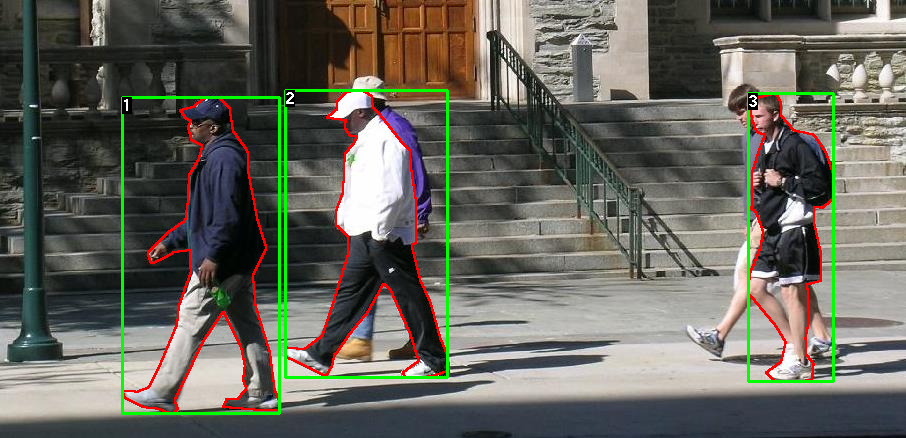
\includegraphics[width=7cm]{graphics/PennPed00015_1.png} }}%
    \qquad
    \subfloat[\centering Mask của hình ảnh]{{
\includegraphics[width=7cm]{graphics/PennPed00015_2.png} }}
    \caption{Một ví dụ trong bộ dữ liệu}
    \label{fig:example}
\end{figure}
\subsection{Thực hành}
\subsubsection{HOG+SVM}
Bài toán áp dụng phương pháp HOG+SVM được thực hiện thông qua ba giai đoạn: tiền xử lý dữ liệu, training và detecting.

Với giai đoạn traning, mô hình sẽ được huấn luyện qua các bước:
\begin{itemize}[noitemsep, topsep=0pt, leftmargin=1.25em, label={$-$}]
    \item Bước 1: Chuẩn bị dữ liệu đào tạo.
    \item Bước 2: Trích xuất đặc trưng HOG.
    \item Bước 3: Huấn luyện SVM phân loại hình ảnh trong bộ dữ liệu đào tạo.
\end{itemize}

Đối với giai đoạn detecting:
\begin{itemize}[noitemsep, topsep=0pt, leftmargin=1.25em, label={$-$}]
    \item Bước 1: Chuẩn bị dữ liệu test khác với dữ liệu đào tạo.
    \item Bước 2: Sử dụng sliding windows trượt qua từng vùng ảnh.
    \item Bước 3: Trích xuất đặc trưng HOG trong từng vùng ảnh.
    \item Bước 4: Phân loại với mô hình SVM đã được đào tạo trong phần training.
\end{itemize}

Có thể hình dung 2 giai đoạn trên qua hình ảnh dưới đây \cite{HOG&SVMped}:   
\graphicspath{{figures/}}
\begin{figure}[h!]
  \centering
  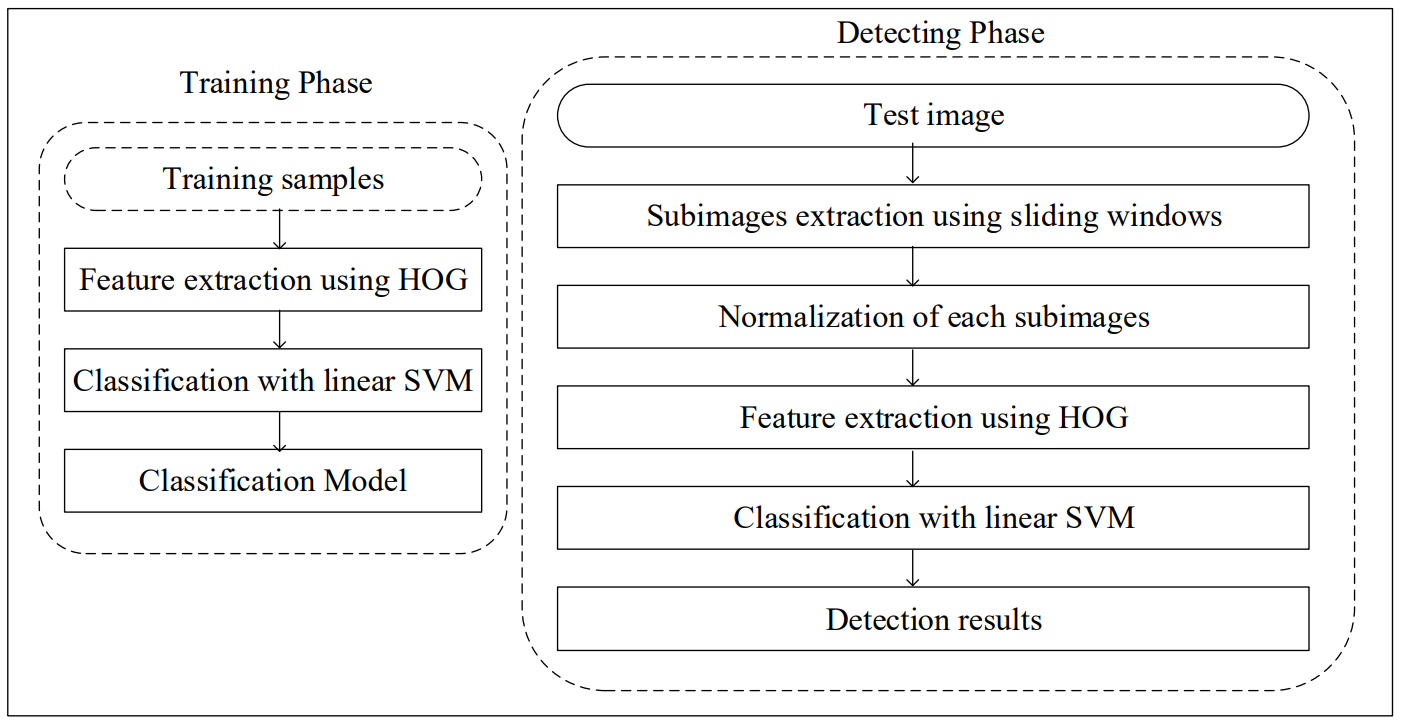
\includegraphics[scale=0.4]{graphics/detectingphaseofHOGSVM.png}
  \caption{Tóm tắt hai giai đoạn traning và detecting của model HOG+SVM.}
\end{figure}

Để hiểu rõ hơn về các bước ở mỗi giai đoạn, chúng ta sẽ đi vào chi tiết qua từng mục dưới đây.
\paragraph{Giai đoạn tiền xử lý dữ liệu\\}
Dataset sử dụng chứa các bức ảnh chứa ít nhất một người đi bộ. Tuy nhiên, vì HOG+SVM là một phương pháp sử dụng mô hình phân loại, chúng ta cần tạo ra tập positive và negative sample set từ dữ liệu huấn luyện. Trong trường hợp này, ta sử dụng 170 bức ảnh trong dataset và có 345 người đi bộ đã được dán nhãn từ dataset.

\textbf{Tạo positive samples} - Đầu tiên, ta đọc các ảnh từ dataset và bounding box (hộp giới hạn) đã được cung cấp. Bước tiếp theo là sử dụng bounding box như ranh giới để lấy các vùng có diện tích bên trong bounding box làm positive sample. Các positive sample này được lưu vào thư mục positive samples. Positive samples là các vùng trong ảnh được xác định là chứa người đi bộ.

\textbf{Tạo negative samples} - Tương tự như bước trước, ta đọc các ảnh từ dataset. Sử dụng hàm detectMultiScale của HOG để xác định các vùng chứa người đi bộ. Với mỗi vùng đã xác định, ta sử dụng sliding window để duyệt qua từng vùng trên từng ảnh đầu vào. Nếu vùng đó trùng với bounding box của detectMultiScale, ta bỏ qua vùng đó và tiếp tục với vùng khác. Ngược lại, nếu vùng không trùng với bounding box, ta lấy vùng đó làm ảnh nền/negative sample. Các negative sample này sau đó được lưu vào thư mục negative samples. Negative samples là các vùng trong ảnh không chứa người đi bộ. Do số lượng negative samples rất lớn so với positive samples, nhóm đã giới hạn lại số lượng negative samples là 800.

\graphicspath{{figures/}}
\begin{figure}[h!]
  \centering
  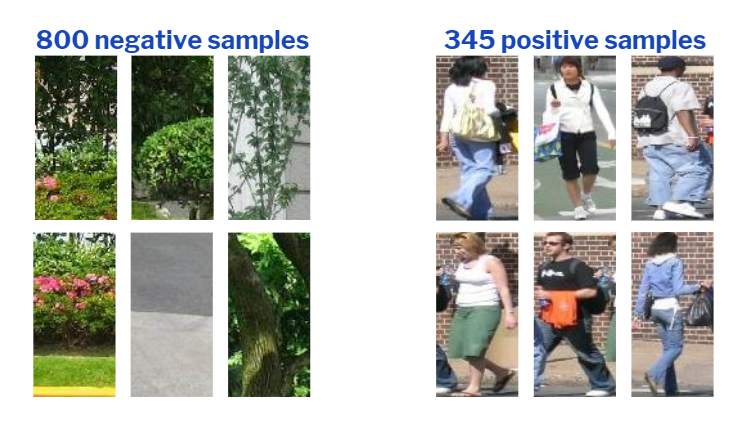
\includegraphics[scale=0.5]{graphics/data-prep.png}
  \caption{Kết quả của giai đoạn tiền xử lí dữ liệu}
\end{figure}

Qua giai đoạn tiền xử lí dữ liệu này, nhóm đã tạo thành hai tập dữ liệu con: positive samples và negative samples. Tỉ lệ của positive và negative samples lần lượt là 345 và 800, tạo ra tập dữ liệu mất cân bằng (imbalanced dataset). Tuy vậy tỉ lệ này lại sát với thực tế, khi mà số lượng người đi bộ trong các bức ảnh là không nhiều và phần lớn vùng diện tích của bức ảnh là nền. Các tập dữ liệu này sẽ được sử dụng trong giai đoạn huấn luyện mô hình SVM để phân loại và nhận dạng người đi bộ trong ảnh.
\paragraph{Giai đoạn training\\}
Trong phần này, model SVM sẽ được training qua chi tiết các bước:
\begin{itemize}[noitemsep, topsep=0pt, leftmargin=1.25em ]
    \item Bước 1: Chuẩn bị dữ liệu:
    \begin{itemize}[noitemsep, topsep=0pt, leftmargin=1.5em, label={$-$}]
        \item Thu thập tập dữ liệu chứa các ảnh với người đi bộ và các ảnh không chứa người đi bộ với kích thước 64x128 như phần tiền xử lý dữ liệu đã nói phía trên.
        \item Gán nhãn dữ liệu: 800 tấm ảnh negative sẽ được gán nhãn là 0, 345 tấm ảnh người positive được gán nhãn là 1.
    \end{itemize}
    \item Bước 2: Trích xuất đặc trưng HOG:
    \begin{itemize}[noitemsep, topsep=0pt, leftmargin=1.5em, label={$-$}]
        \item Sử dụng phương pháp HOG (Histogram of Oriented Gradients) để trích xuất đặc trưng từ các hình ảnh trong bộ dữ liệu đào tạo.
    \end{itemize}
    \item Bước 3: Huấn luyện SVM phân loại hình ảnh trong bộ dữ liệu đào tạo:
    \begin{itemize}[noitemsep, topsep=0pt, leftmargin=1.5em, label={$-$}]
        \item Kết hợp hai bộ ảnh đã được tính đặc trưng HOG là positive và negative lại với nhau để chia tập dữ liệu thành train và test. Với tỉ lệ 8:2 ta có được tập train là 915 hình ảnh và tập test là 230 hình ảnh.
        \item Sử dụng các đặc trưng HOG đã được trích xuất từ bước trước đó và nhãn tương ứng để huấn luyện một mô hình SVM với hai tập dữ liệu train và test.
    \end{itemize}
\end{itemize}

Sau giai đoạn traning, chúng ta sẽ có được model SVM đã train sử dụng nó để detect người đi bộ trong giai đoạn tiếp theo.
\paragraph{Giai đoạn deteting\\}
Với giai đoạn detecting, ta sẽ có thêm một số khái niệm cần chú ý, trước tiên ta sẽ đi qua chi tiết các bước:
\begin{itemize}[noitemsep, topsep=0pt, leftmargin=1.25em ]
    \item Bước 1: Chuẩn bị dữ liệu test khác với dữ liệu đào tạo:
    \begin{itemize}[noitemsep, topsep=0pt, leftmargin=1.5em, label={$-$}]
        \item Dữ liệu test cho phần phát hiện đối tượng này là các hình ảnh chứa 1 hoặc nhiều người đi bộ để kiểm tra model phát hiện người đi bộ trong hình ảnh.
    \end{itemize}
    \item Bước 2: Sử dụng \textbf{sliding windows} trượt qua từng vùng ảnh:
        \begin{itemize}[noitemsep, topsep=0pt, leftmargin=1.5em, label={$-$}]
            \item Áp dụng kỹ thuật \textbf{sliding windows} để chia nhỏ các hình ảnh trong bộ dữ liệu test thành các vùng nhỏ có kích thước 64x128.
            \item \textbf{Sliding windows} - là kĩ thuật sử dụng để quét qua toàn bộ hình ảnh bằng cách di chuyển một cửa sổ trượt có kích thước cố định qua từng vị trí trên ảnh, sau đó tăng kích thước cửa sổ với tỷ lệ được định nghĩa rồi tiếp tục quét cho đến khi kích thước cửa sổ được tăng bằng với kích thước ảnh. Bắt đầu từ góc trên bên trái của ảnh, cửa sổ trượt được di chuyển qua từng vị trí trên ảnh một cách tuần tự. Cửa sổ có thể được di chuyển theo bước nhảy (stride) cố định hoặc bước nhảy có thể được điều chỉnh tùy thuộc vào yêu cầu của bài toán.
            \graphicspath{{figures/}}
                \begin{figure}[h!]
                  \centering
                  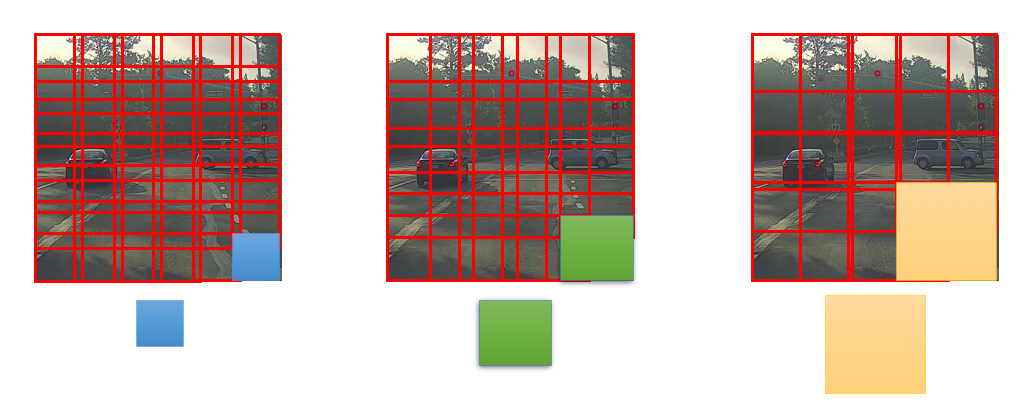
\includegraphics[scale=0.35]{graphics/slidingw.png}
                  \caption{Cách sliding window hoạt động trên một hình ảnh.}
                \end{figure}
            \item Việc chia nhỏ ảnh thành các vùng nhỏ này giúp xác định vị trí có thể xuất hiện người đi bộ trong ảnh.
        \end{itemize}
    \item Bước 3: Trích xuất đặc trưng HOG trong từng vùng ảnh:
    \begin{itemize}[noitemsep, topsep=0pt, leftmargin=1.5em, label={$-$}]
        \item Áp dụng phương pháp HOG để trích xuất đặc trưng từ từng vùng ảnh nhỏ thu được từ bước trước.
        \item Việc trích xuất đặc trưng HOG giúp tạo ra một biểu diễn số học của mỗi vùng ảnh, giúp phân loại xem có người đi bộ trong vùng đó hay không.
    \end{itemize}
    \item Bước 4: Phân loại với mô hình SVM đã được đào tạo trong phần training:
    \begin{itemize}[noitemsep, topsep=0pt, leftmargin=1.5em, label={$-$}]
        \item Sử dụng mô hình SVM đã được huấn luyện trong phần training để phân loại các vùng ảnh thu được từ bước trước. 
        \item Mô hình sẽ phân loại các ảnh con được quét qua bởi sliding window là ảnh nền hay ảnh con người theo những gì được học ở giai đoạn training.
    \end{itemize}
\end{itemize}
Quá trình trượt qua toàn bộ hình ảnh và áp dụng phân loại trên từng cửa sổ được lặp lại cho đến khi đã duyệt qua tất cả các vị trí trên ảnh. Cuối cùng, sử dụng kỹ thuật \textbf{non\_max\_suppression} để loại bỏ các khu vực overlap và chỉ giữ lại kết quả phân loại cuối cùng.
    \begin{itemize}[noitemsep, topsep=0pt, leftmargin=1.5em, label={$-$}]
        \item Một khái niệm nữa được dùng trong giai đoạn này đó là \textbf{non\_max\_suppression}. 
        \item \textbf{Non-maximum suppression (NMS)} - một kỹ thuật được sử dụng trong xử lý ảnh để loại bỏ trùng lặp và chọn lọc các đối tượng có độ tin cậy cao. Khi sử dụng kỹ thuật sliding window để phát hiện đối tượng trong ảnh, có thể xảy ra tình huống nhiều cửa sổ trượt chồng lấp lên nhau và phát hiện cùng một đối tượng. Điều này dẫn đến việc nhận dạng trùng lặp và tạo ra nhiều kết quả phát hiện không cần thiết. Để giảm hiện tượng này, ta sử dụng kỹ thuật non-maximum suppression.
        \graphicspath{{figures/}}
            \begin{figure}[h!]
            \centering
            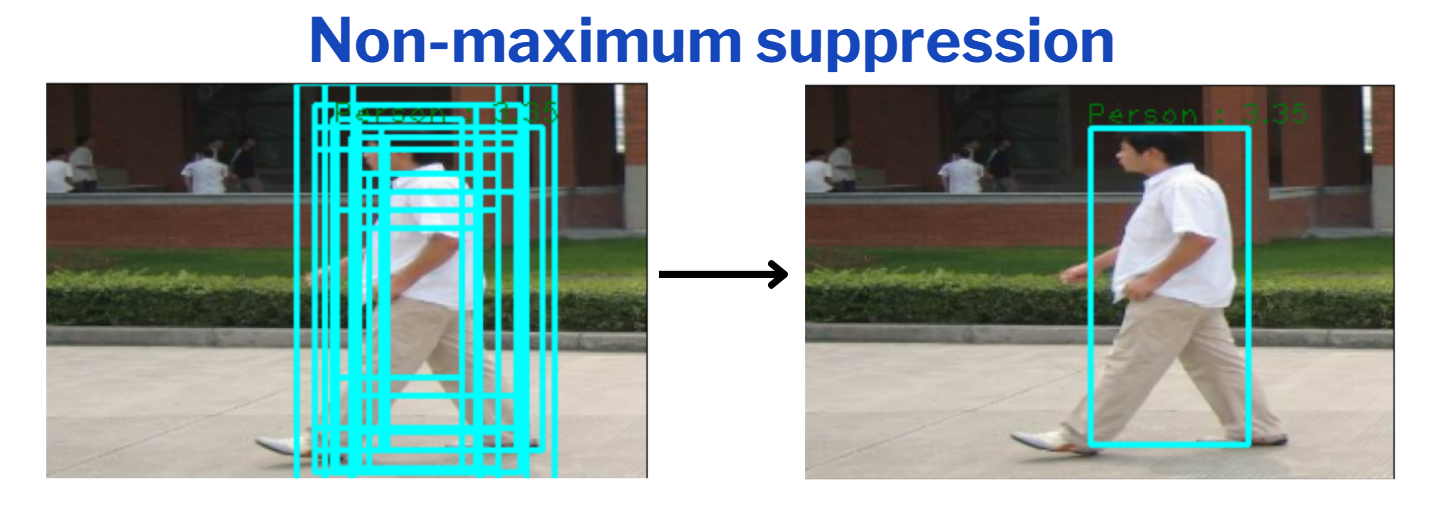
\includegraphics[scale=0.35]{graphics/NMS.png}
            \caption{NMS loại bỏ phát hiện dư trùng lặp, giữ lại phát hiện đáng tin cậy.}
        \end{figure}
    \end{itemize}
Cuối cùng, vẽ các hộp giới hạn xung quanh các khu vực dành cho người đi bộ được phát hiện và được xóa trùng lặp bởi NMS. Hình ảnh output nhận được sẽ là hình ảnh phát hiện người đi bộ bằng các bounding box bao quanh vùng phát hiện đó.

\subsubsection{Faster R-CNN}
\paragraph{Chuẩn bị bộ dữ liệu Penn-FundanFundan\\}

Phương thức getitem sẽ trả về: image là một PIL Image có kích thước (H, W) và target là một từ điển chứa các trường sau đây:
\begin{itemize}[noitemsep, topsep=0pt, leftmargin=1.25em, label={$-$}]
    \item boxes (FloatTensor[N, 4]): tọa độ của N bounding boxes trong định dạng [x0, y0, x1, y1], có giá trị từ 0 đến W và 0 đến H.
    \item labels (Int64Tensor[N]): nhãn cho mỗi bounding box. Giá trị 0 luôn đại diện cho lớp nền (background).
    \item image\_id (Int64Tensor[1]): một định danh hình ảnh. Nó là duy nhất giữa tất cả các hình ảnh trong bộ dữ liệu và được sử dụng trong quá trình đánh giá.
    \item area (Tensor[N]): Diện tích của bounding box được sử dụng trong quá trình đánh giá với các tiêu chí COCO, để phân tách điểm số tiêu chí cho các bounding box nhỏ, vừa và lớn.
    \item iscrowd (UInt8Tensor[N]): Các instance với iscrowd=True sẽ được bỏ qua trong quá trình đánh giá.
\end{itemize}
\begin{figure}[h!]
  \centering
  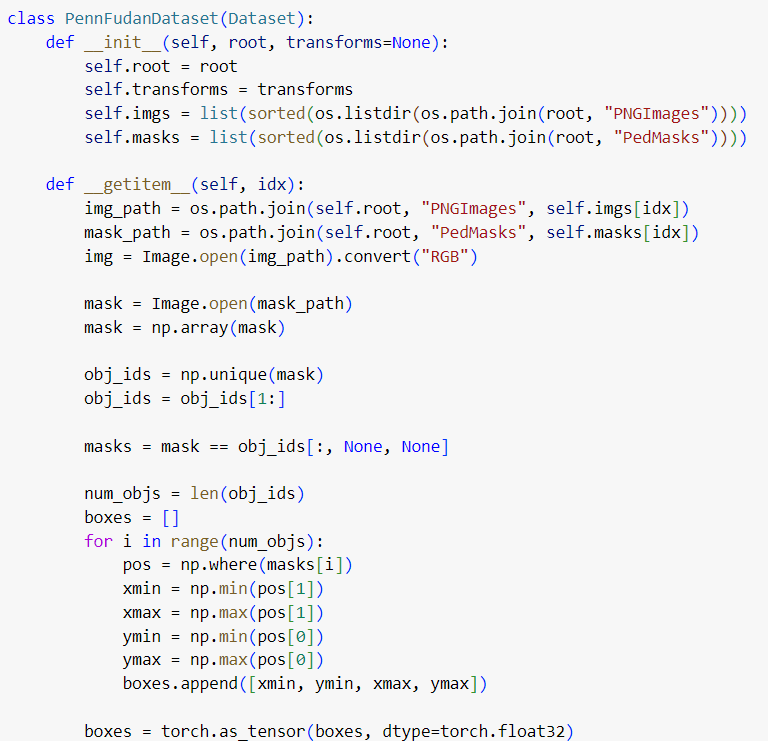
\includegraphics[scale=0.65]{graphics/loaddata.png}
  \caption{Hàm để load bộ dữ liệu Penn-Fundan}
\end{figure}
\pagebreak
\paragraph{Xây dựng mô hình\\}
Nhóm chúng em đã lựa chọn như sau:
\begin{itemize}[noitemsep, topsep=0pt, leftmargin=1.25em, label={$-$}]
    \item backbone: sử dụng mô hình mạng nơ-ron tiền huấn luyện MobileNetV2. Mô hình này sẽ được sử dụng để trích xuất đặc trưng từ ảnh đầu vào.
    \item AnchorGenerator được sử dụng để tạo ra các vùng đề xuất trên feature map để đề xuất các vùng có khả năng chứa đối tượng cao.
    \item MultiScaleRoIAlign được sử dụng để pooling features từ feature map theo vùng đề xuất (region of interest - ROI) để chuẩn bị đầu vào cho lớp classification và regression của mô hình.
    \item Faster R-CNN được cấu hình để nhận diện 2 lớp đối tượng: có người đi bộ và background (num\_classes=2)
\end{itemize}

\pagebreak

\begin{figure}[h!]
  \centering
  \subfloat{{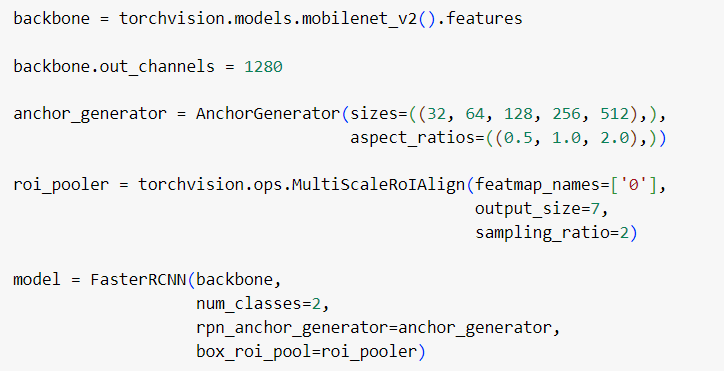
\includegraphics[scale=0.7]{graphics/backbone.png} }}
  \qquad
  \subfloat{{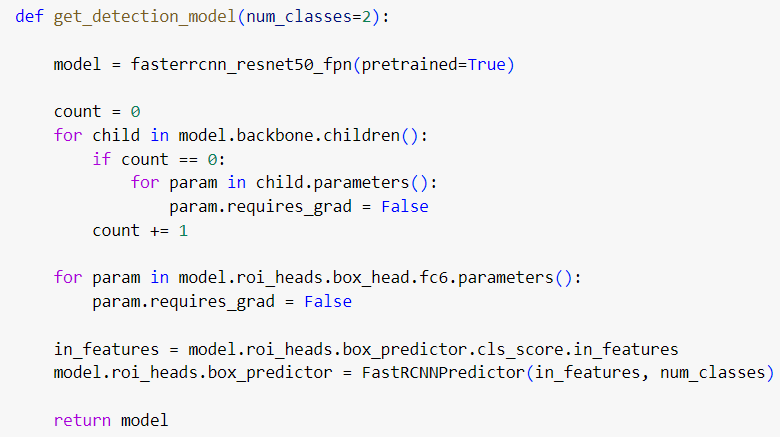
\includegraphics[scale=0.7]{graphics/model.png} }}
  \caption{Code xây dựng mô hình Faster R-CNN}
\end{figure}

Ta thực hiện hàm transform để biến đổi mỗi hình ảnh đầu vào sang định dạng phù hợp để mô hình các mạng nơ-ron của PyTorch có thể xử lý được. 
\begin{figure}[h!]
  \centering
  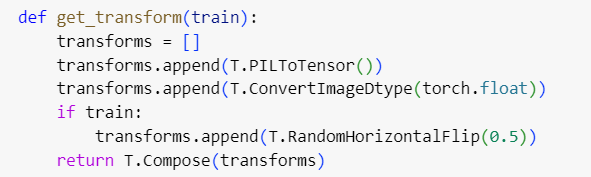
\includegraphics[scale=0.65]{graphics/transform.png}
  \caption{Hàm transform}
\end{figure}

\paragraph{Chia tập train và test\\}
Tiếp theo ta chia dataset thành hai tập train và test để sử dụng cho việc huấn luyện và đánh giá mô hình. Trong phần thực nghiệm này, nhóm chia với tỉ lệ 0.7 nghĩa là 70\% dữ liệu sử dụng cho tập huấn luyện.

\pagebreak

\begin{figure}[h!]
  \centering
  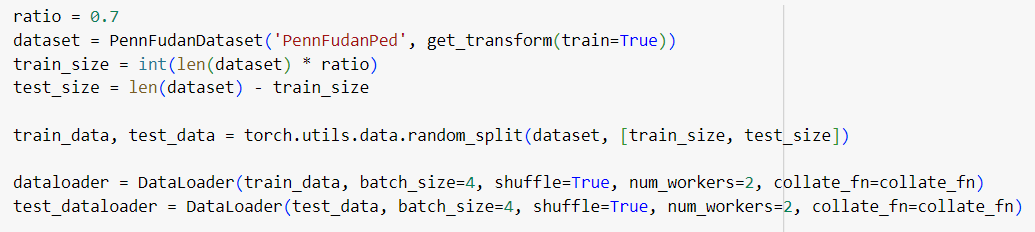
\includegraphics[scale=0.65]{graphics/split.png}
  \caption{Chia dataset bằng train\_test\_split}
\end{figure}

\paragraph{Lựa chọn các hyperparameters\\}
Ở phần này, nhóm chỉ sẽ thực nghiệm với các giá trị learning rate (lr) $\in \{0.004, 0.005, 0.006\}$ để đánh giá mô hình khi learning rate thay đổi trong các giá trị này. Các giá trị tham số khác được tham khảo từ thư viện PyTorch.
\begin{figure}[h!]
  \centering
  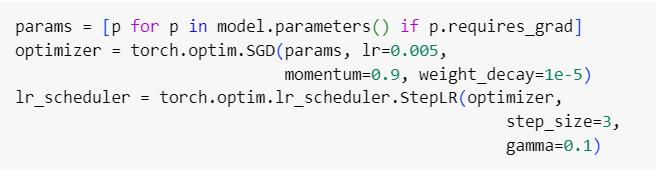
\includegraphics[scale=0.8]{graphics/params.png}
  \caption{Lựa chọn các hyperparameters}
\end{figure}

\paragraph{Huấn luyện mô hình\\}
Với mỗi epoch ta tính tổng giá trị loss và in ra để quan sát.
\begin{figure}[h!]
  \centering
  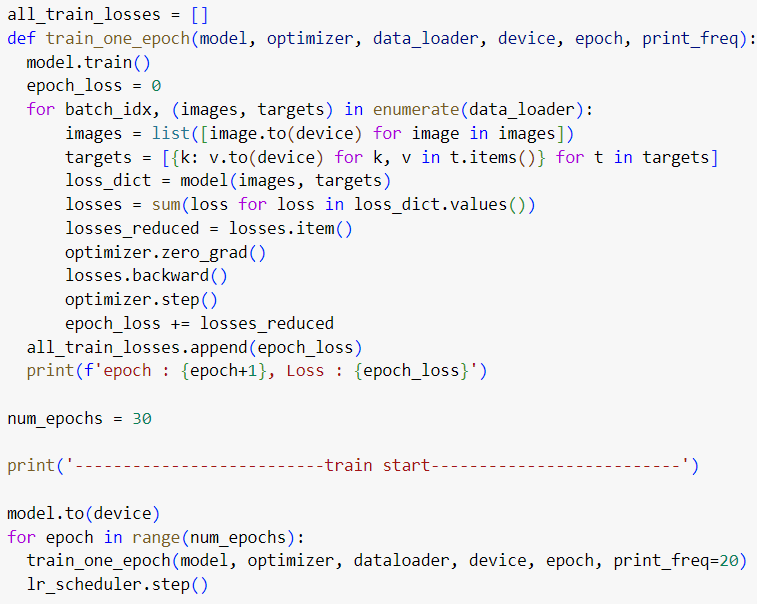
\includegraphics[scale=0.7]{graphics/train.png}
  \caption{Huấn luyện mô hình với 30 epochs}
\end{figure}
\subsection{Kết quả}
\subsubsection{Đánh giá bằng độ đo mAP}
\begin{table}[ht]
   \begin{center}
    \caption{Kết quả mAP với threshold=0.5}
    \begin{tabular}{c | c | *3c}
    \toprule
    Mô hình &  HOG+SVM  & \multicolumn{3}{c}{Faster R-CNN}\\
    \hline
    {}   &             & lr=0.004  & lr=0.005 & lr=0.006\\
    mAP   &      0.271      & 0.591  & 0.604 & 0.619\\
    \bottomrule
    \end{tabular}
  \end{center}
\end{table}
\subsubsection{Trên tập test}
\textbf{HOG+SVM}\\

\begin{figure}[h!]
  \centering
  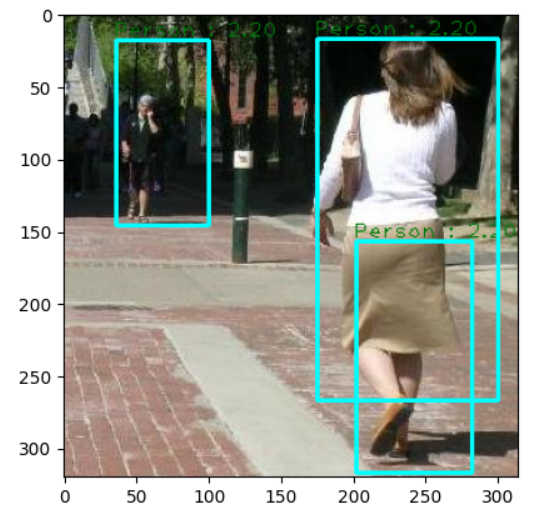
\includegraphics[scale=0.7]{graphics/testhogsvm.png}
  \caption{Kết quả mô hình HOG+SVM}
\end{figure}

Có thể thấy, HOG+SVM phát hiện người đi bộ vẫn chưa được chính xác. Một phần là vì bộ dữ liệu train model vẫn còn thấp, nhưng ta vẫn thấy được sự tương đối của mô hình này trong phát hiện đối tượng ở đây là người đi bộ.\\ 

\textbf{Faster R-CNN}
\pagebreak

\begin{figure}[h!]
  \centering
  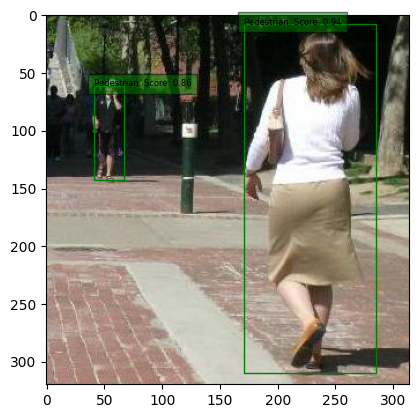
\includegraphics[scale=0.7]{graphics/test_0004.png}
  \caption{Kết quả mô hình Faster R-CNN trên tập test với r=0.004}
\end{figure}

\begin{figure}[h!]
  \centering
  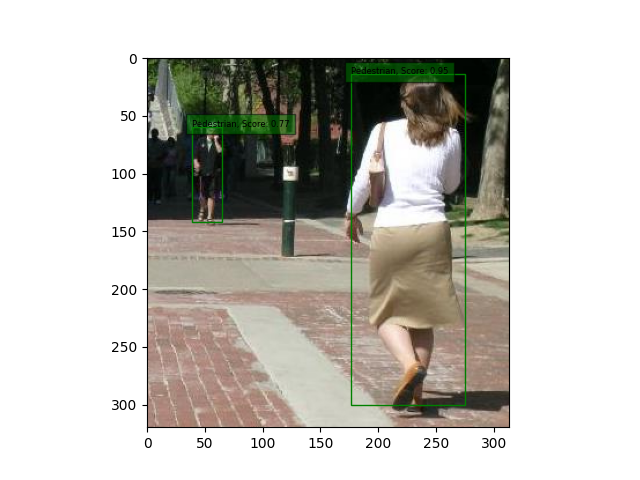
\includegraphics[scale=0.7]{graphics/test_0005.png}
  \caption{Kết quả mô hình Faster R-CNN trên tập test với lr=0.005}
\end{figure}

\pagebreak

\begin{figure}[h!]
  \centering
  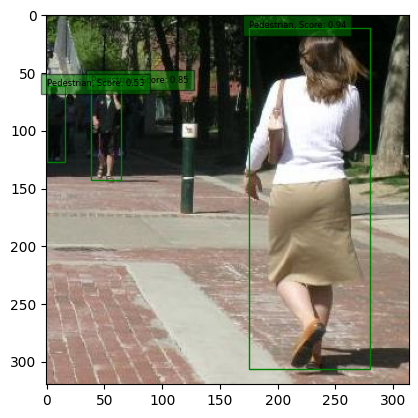
\includegraphics[scale=0.7]{graphics/test_0006.png}
  \caption{Kết quả mô hình Faster R-CNN trên tập test với lr=0.006}
\end{figure}

Theo kiến thức và thị giác của con người, ta có thể thấy rằng giữa ba giá trị của learning\_rate thì lr=0.006 cho kết quả tốt hơn so với hai giá trị còn lại vì detect được một người bị khuất trong bóng râm trong bức hình.\\

\subsubsection{Trên hình ảnh số bất kỳ}
\textbf{HOG+SVM}

\begin{figure}[h!]
  \centering
  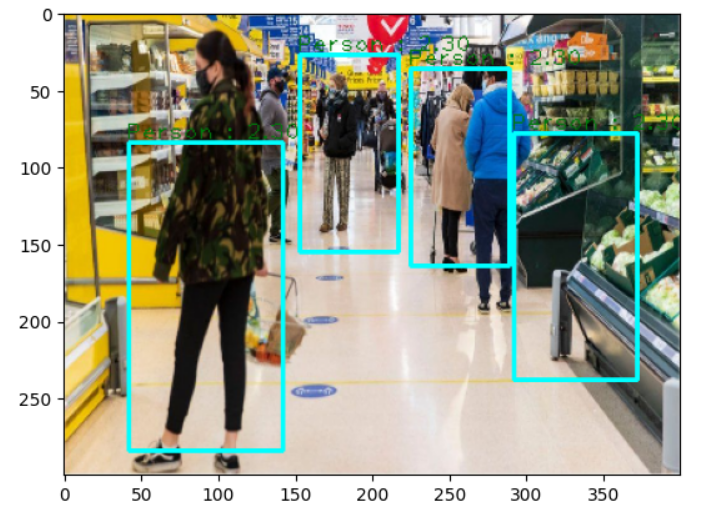
\includegraphics[scale=0.55]{graphics/rshogsvm0.png}
  \caption{Kết quả trên một hình ảnh trong siêu thị của HOG+SVM}
\end{figure}

\begin{figure}[h!]
  \centering
  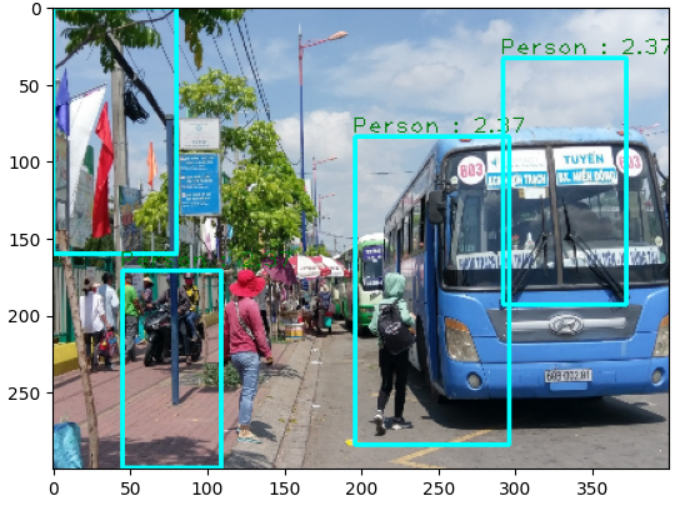
\includegraphics[scale=0.55]{graphics/rshogsvm1.png}
  \caption{Kết quả trên một hình ảnh ở bến xe buýt Suối Tiên của HOG+SVM}
\end{figure}
\pagebreak

\textbf{Faster R-CNN}

\begin{figure}[h!]
  \centering
  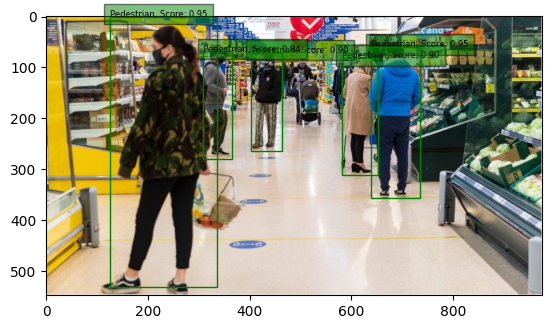
\includegraphics[scale=0.7]{graphics/demo1.png}
  \caption{Kết quả trên một hình ảnh trong siêu thị của Faster R-CNN với lr=0.006}
\end{figure}

\begin{figure}[h!]
  \centering
  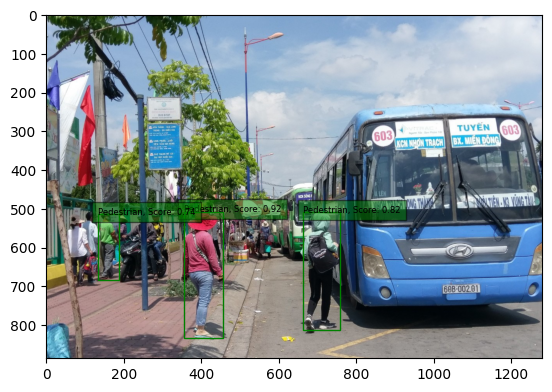
\includegraphics[scale=0.7]{graphics/demo2.png}
  \caption{Kết quả trên một hình ảnh ở bến xe buýt Suối Tiên của Faster R-CNN với lr=0.005}
\end{figure}
\subsection{Triển khai mô hình bằng Streamlit}
Trong đoạn mã, trước tiên chúng ta cần import các thư viện cần thiết như Streamlit, torch, joblib, cv2, numpy và các module khác.

Sau đó, chúng ta có hai hàm chính: faster\_rcnn\_detection và hog\_svm\_detection.

Trong hàm faster\_rcnn\_detection, ta mở ảnh đầu vào và khởi tạo mô hình Faster R-CNN pre-trained. Mô hình này đã được tinh chỉnh để nhận dạng người đi bộ. Sau đó, ta tải trọng số đã được huấn luyện từ tệp model\_30.pt. Tiếp theo, ta sử dụng mô hình để dự đoán trên ảnh và lấy ra các hộp giới hạn (bounding boxes) được dự đoán, nhãn tương ứng và độ tin cậy (score) của các nhãn. Chúng ta sử dụng ngưỡng (threshold) 0.8 để lọc các dự đoán có độ tin cậy cao. Cuối cùng, chúng ta vẽ các hộp giới hạn và thông tin nhãn lên ảnh và hiển thị ảnh kết quả.

Trong hàm hog\_svm\_detection, ta tải mô hình SVM đã được huấn luyện từ tệp models.dat. Tiếp theo, chúng ta tiến hành xử lý ảnh đầu vào bằng phương pháp HOG (Histogram of Oriented Gradients) và duyệt qua các cửa sổ trượt (sliding windows) trên ảnh. Với mỗi cửa sổ, ta rút trích đặc trưng HOG và sử dụng mô hình SVM để dự đoán xem cửa sổ đó có chứa người đi bộ hay không. Nếu dự đoán là positive, ta lưu lại thông tin về vị trí và độ tin cậy của cửa sổ. Tiếp theo, chúng ta sử dụng non-maximum suppression để loại bỏ các hộp giới hạn trùng lắp và chỉ giữ lại hộp giới hạn có độ tin cậy cao nhất. Cuối cùng, chúng ta vẽ các hộp giới hạn đã lựa chọn lên ảnh và hiển thị ảnh kết quả.

Cuối cùng, trong hàm main, chúng ta sử dụng Streamlit để tạo giao diện người dùng. Người dùng có thể tải lên một tệp ảnh và xem kết quả phát hiện người đi bộ sử dụng cả hai phương pháp Faster R-CNN và HOG+SVM. Kết quả sẽ được hiển thị trên trang web Streamlit.

Qua đó, việc triển khai mô hình trên Streamlit cho phép người dùng tải lên ảnh và trực quan hóa kết quả phát hiện người đi bộ sử dụng hai phương pháp khác nhau, giúp phân tích và so sánh hiệu suất của các phương pháp trong bài toán này.

\begin{figure}[h!]
  \centering
  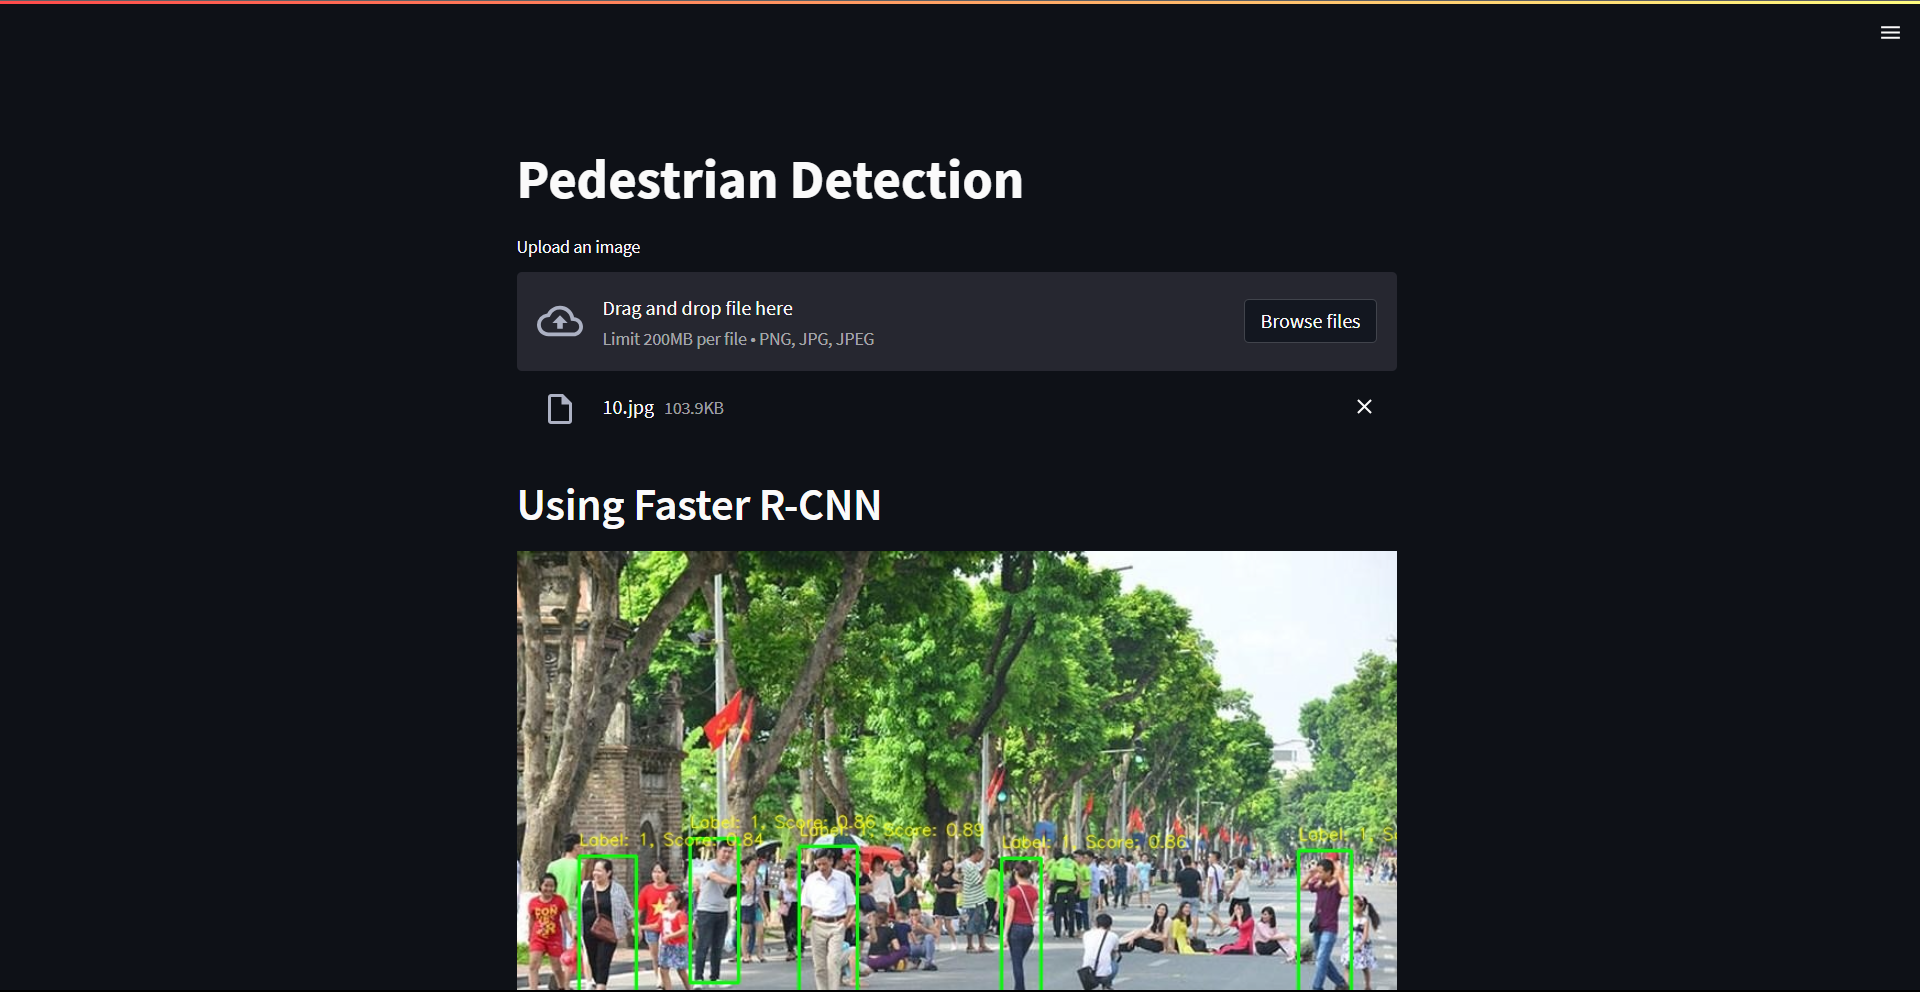
\includegraphics[scale=0.35]{graphics/streamlit.png}
  \caption{Deploy mô hình trên local host website bằng Streamlit}
\end{figure}
\subsection{Source code}
Source code của đồ án này đã được nhóm đăng trên Github repository: \href{https://github.com/blkhanhlinh/pedestrian-detection}{\underline{pedestrian-detection}}

Repository này chứa các tệp tin và mã nguồn liên quan đến bài toán nhận diện người đi bộ đã được đề cập trong báo cáo. Bao gồm cách thức mà nhóm đã thực hiện cho mô hình HOG + SVM cũng như Faster R-CNN trên tập dữ liệu PennFudan Pedestrian. Những tệp tin và mã nguồn này có thể được sử dụng làm tài liệu tham khảo cho các nhiệm vụ tương tự hoặc như một điểm khởi đầu để thực hiện các phương pháp nhận diện người đi bộ khác. Bất kỳ ai quan tâm đều có thể truy cập repository và làm theo hướng dẫn trong tệp README để cài đặt và chạy mô hình trên máy tính của mình. 

\pagebreak
\bibliographystyle{unsrt}
\bibliography{refs}
\end{document}